\documentclass[11pt,a4paper]{article}

% ---- Packages ----
\usepackage[utf8]{inputenc}
\usepackage[T1]{fontenc}
\usepackage[english]{babel}

\usepackage[margin=1.1in]{geometry}
\usepackage{amsmath, amssymb, amsthm, mathtools}
\usepackage{booktabs, array}
\usepackage{enumitem}
\usepackage{xcolor}
\usepackage{graphicx}
\usepackage{epigraph}
\usepackage{csquotes}
\usepackage{listings}
\usepackage{tikz}
\usetikzlibrary{arrows.meta, positioning, shapes.geometric, shapes.misc,
                fit, calc, backgrounds, decorations.pathreplacing,
                patterns, matrix}
\usepackage{pgfplots}
\pgfplotsset{compat=1.18}

\usepackage[colorlinks=true, linkcolor=black!70!blue,
            citecolor=black!70!blue, urlcolor=black!40!blue]{hyperref}

% ---- Code listings (restrained, matches the rest of the notes) ----
\lstset{
    basicstyle=\small\ttfamily,
    keywordstyle=\bfseries,
    commentstyle=\itshape\color{black!60},
    stringstyle=\color{black!70},
    language=Python,
    breaklines=true,
    frame=single,
    rulecolor=\color{black!25},
    xleftmargin=1em,
    xrightmargin=1em,
    showstringspaces=false
}

% ---- Theorem environments ----
\theoremstyle{definition}
\newtheorem{definition}{Definition}[section]
\newtheorem{example}[definition]{Example}

\theoremstyle{remark}
\newtheorem*{remark}{Remark}
\newtheorem*{aside}{Aside}
\newtheorem*{observation}{Observation}

\theoremstyle{plain}
\newtheorem{proposition}[definition]{Proposition}

% ---- Epigraph style ----
\setlength{\epigraphwidth}{0.6\textwidth}
\renewcommand{\epigraphflush}{flushright}
\renewcommand{\textflush}{flushright}
\renewcommand{\epigraphsize}{\small\itshape}

% ---- Small conveniences ----
\newcommand{\todo}[1]{\textcolor{red!70!black}{\textbf{[TODO: #1]}}}
\DeclareMathOperator*{\argmin}{arg\,min}
\newcommand{\grad}{\nabla}
\newcommand{\LL}{\mathcal{L}}
\newcommand{\DD}{\mathcal{D}}
\DeclareMathOperator*{\AllReduce}{AllReduce}
\DeclareMathOperator*{\AllGather}{AllGather}
\DeclareMathOperator*{\ReduceScatter}{ReduceScatter}
\DeclareMathOperator{\softmax}{softmax}
\DeclareMathOperator{\GeLU}{GeLU}
\DeclareMathOperator{\ReLU}{ReLU}
\DeclareMathOperator{\LayerNorm}{LayerNorm}

% ---- Title ----
\title{\textbf{Efficient Deep Learning Systems} \\[0.3em]
       \large Lecture 4 --- Memory-Efficient Training and Model Parallelism: \\
       Checkpointing, Offloading, Pipeline and Tensor Parallelism, and Sharding}
\author{Lecture notes}
\date{}

\begin{document}
\sloppy
\maketitle

\begin{abstract}
\noindent
These notes trace the architectural and algorithmic ideas that enable the
training of neural networks whose parameters, activations, and optimizer
states exceed the memory of any single accelerator. We begin with
collective communication primitives---the grammar of distributed
training---and proceed through gradient accumulation, checkpointing,
offloading, pipeline parallelism, tensor parallelism, sequence
parallelism, and mixtures of experts. The concluding sections examine
fully sharded data parallelism, automated parallelism, and the internals
of PyTorch's autograd machinery that make all of this expressible.
\end{abstract}

\tableofcontents
\bigskip
\hrule
\bigskip

%%%%%%%%%%%%%%%%%%%%%%%%%%%%%%%%%%%%%%%%%%%%%%%%%%%%%%%%%%%%%%%%%%%%%%%%
\section{Prologue: Why Parallelism Matters}
%%%%%%%%%%%%%%%%%%%%%%%%%%%%%%%%%%%%%%%%%%%%%%%%%%%%%%%%%%%%%%%%%%%%%%%%

In prior discussions we established the foundations of
\emph{data-parallel} deep learning, in which a dataset is partitioned
across multiple computing units and gradient updates are averaged to
accelerate training. Data parallelism is elegant and nearly free when the
model fits on a single device. It is also, increasingly, insufficient.

The empirical trajectory of the past decade has been unambiguous: across
image classification, machine translation, and generative modelling,
model quality improves monotonically with parameter count. Models
exceeding a trillion parameters are now routinely deployed. The schematic
below summarises this scaling phenomenon; the original plots appear in the
GPipe paper.\footnote{Huang et al., \textit{GPipe}:
\url{https://arxiv.org/abs/1811.06965}.}

\begin{center}
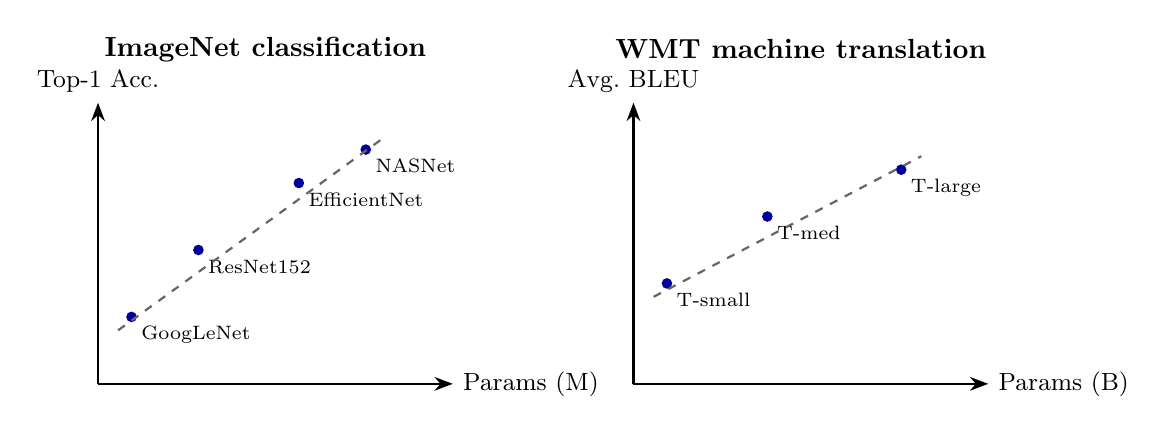
\begin{tikzpicture}[scale=0.85, >=Stealth]
% --- Image Classification panel ---
\begin{scope}[shift={(0,0)}]
    \draw[thick, ->] (0,0) -- (5.3,0) node[right] {\small Params (M)};
    \draw[thick, ->] (0,0) -- (0,4.2) node[above] {\small Top-1 Acc.};
    \node at (2.5, 5) {\textbf{ImageNet classification}};
    \filldraw[blue!60!black] (0.5, 1.0) circle (2pt) node[below right, font=\scriptsize, text=black] {GoogLeNet};
    \filldraw[blue!60!black] (1.5, 2.0) circle (2pt) node[below right, font=\scriptsize, text=black] {ResNet152};
    \filldraw[blue!60!black] (3.0, 3.0) circle (2pt) node[below right, font=\scriptsize, text=black] {EfficientNet};
    \filldraw[blue!60!black] (4.0, 3.5) circle (2pt) node[below right, font=\scriptsize, text=black] {NASNet};
    \draw[dashed, thick, black!60] (0.3, 0.8) -- (4.3, 3.7);
\end{scope}
% --- Machine Translation panel ---
\begin{scope}[shift={(8,0)}]
    \draw[thick, ->] (0,0) -- (5.3,0) node[right] {\small Params (B)};
    \draw[thick, ->] (0,0) -- (0,4.2) node[above] {\small Avg.\ BLEU};
    \node at (2.5, 5) {\textbf{WMT machine translation}};
    \filldraw[blue!60!black] (0.5, 1.5) circle (2pt) node[below right, font=\scriptsize, text=black] {T-small};
    \filldraw[blue!60!black] (2.0, 2.5) circle (2pt) node[below right, font=\scriptsize, text=black] {T-med};
    \filldraw[blue!60!black] (4.0, 3.2) circle (2pt) node[below right, font=\scriptsize, text=black] {T-large};
    \draw[dashed, thick, black!60] (0.3, 1.3) -- (4.3, 3.4);
\end{scope}
\end{tikzpicture}
\par\smallskip
{\small Schematic of the scaling trend; point positions are illustrative,
not the original data.}
\end{center}

Early Transformer research already hinted that models in the
$2$--$8\,\mathrm{B}$ parameter regime exhibit qualitatively surprising
capabilities. The challenge has correspondingly shifted from \emph{model
design} to \emph{training efficiency}: how does one orchestrate
synchronisation when the model, its gradients, its optimizer states, and
its activations each vie for a finite memory budget?

%%%%%%%%%%%%%%%%%%%%%%%%%%%%%%%%%%%%%%%%%%%%%%%%%%%%%%%%%%%%%%%%%%%%%%%%
\section{Collective Communication: The Grammar of Distributed Training}
\label{sec:collectives}
%%%%%%%%%%%%%%%%%%%%%%%%%%%%%%%%%%%%%%%%%%%%%%%%%%%%%%%%%%%%%%%%%%%%%%%%

\subsection{The \textsc{AllReduce} Primitive}

A cluster performing data-parallel training typically maintains, on each
node, a replica of the model. During an iteration, each replica computes a
local gradient from its shard of the batch, after which the gradients must
be aggregated. This aggregation is the role of the \textsc{AllReduce}
operator.

\begin{definition}[\textsc{AllReduce}]
Given $N$ nodes each holding a tensor $g_i$, an \textsc{AllReduce} with
reduction operator $\oplus$ produces on every node the reduced value
$\bigoplus_{i=1}^{N} g_i$. Summation is by far the most common choice,
though minimum, maximum, and product reductions are supported.
\end{definition}

Though \textsc{AllReduce} has a simple semantic specification, it may be
implemented over many topologies---tree, butterfly, and ring---each
trading latency against bandwidth. What unifies them is a common
workflow: each node first performs a \emph{partial reduction} to minimise
egress traffic, after which data is aggregated across the network until
every node holds the final reduced result.

\subsection{Ring \textsc{AllReduce}}

The ring topology is particularly efficient in bandwidth-optimal regimes.
Nodes are arranged in a closed loop and each communicates only with its
two neighbours. (For how to perform the reduction when GPUs can only talk to their
neighbours, see this
\href{https://tinyurl.com/ring-allreduce-blog}{blog post}; the topology
is also used in \href{https://www.graphcore.ai/}{Graphcore} IPU servers.)

\begin{center}
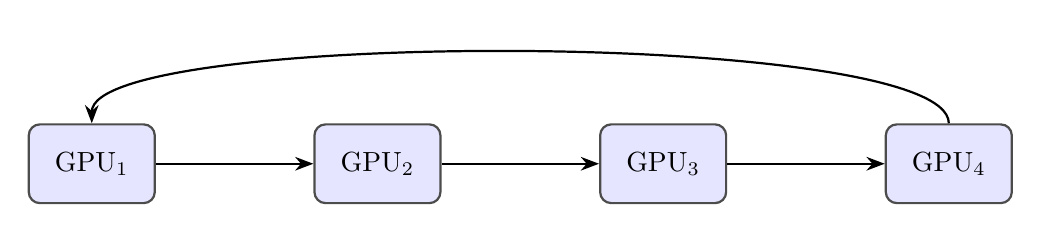
\begin{tikzpicture}[
    node distance=2cm, >=Stealth,
    gpu/.style={rectangle, rounded corners, draw=black!70, thick,
                fill=blue!10, minimum width=1.6cm, minimum height=1cm}
]
    \node[gpu] (gpu1) {GPU$_1$};
    \node[gpu, right=of gpu1] (gpu2) {GPU$_2$};
    \node[gpu, right=of gpu2] (gpu3) {GPU$_3$};
    \node[gpu, right=of gpu3] (gpu4) {GPU$_4$};
    \draw[-Stealth, thick] (gpu1) -- (gpu2);
    \draw[-Stealth, thick] (gpu2) -- (gpu3);
    \draw[-Stealth, thick] (gpu3) -- (gpu4);
    \draw[-Stealth, thick] (gpu4.north) .. controls +(up:1.2cm) and +(up:1.2cm) .. (gpu1.north);
\end{tikzpicture}
\end{center}

\subsection{Decomposition: \textsc{ReduceScatter} and \textsc{AllGather}}

A subtlety worth internalising is that \textsc{AllReduce} is not atomic;
it decomposes naturally into two primitives.

\begin{proposition}[Decomposition of \textsc{AllReduce}]
For any commutative, associative reduction operator $\oplus$,
\begin{equation}
\AllReduce \;=\; \AllGather \circ \ReduceScatter.
\end{equation}
In the first phase each node aggregates a distinct fragment of the global
reduction; in the second phase every node retrieves all fragments, at
which point every node holds the full reduced tensor.
\end{proposition}

Those familiar with \texttt{torch.distributed} will recognise these as
the atomic primitives; \textsc{AllReduce} is itself a convenience.

\begin{observation}
Because \textsc{AllReduce} guarantees that every GPU receives an
\emph{identical} reduced gradient, and because each device applies this
gradient to an identical local copy of the weights, the updated weights
remain bitwise identical across the cluster. No further synchronisation
of parameters is necessary; only of gradients. (This is the all-reduce
SGD scheme of Goyal et al.,
\href{https://arxiv.org/abs/1706.02677}{arXiv:1706.02677}.)
\end{observation}

%%%%%%%%%%%%%%%%%%%%%%%%%%%%%%%%%%%%%%%%%%%%%%%%%%%%%%%%%%%%%%%%%%%%%%%%
\section{Gradient Accumulation: Simulating a Larger Batch}
%%%%%%%%%%%%%%%%%%%%%%%%%%%%%%%%%%%%%%%%%%%%%%%%%%%%%%%%%%%%%%%%%%%%%%%%

Large batches are a practical necessity for stable Transformer training:
a language model may require $16{,}000$ tokens per optimiser step when
the hardware will only admit a handful at a time. \emph{Gradient
accumulation} reconciles this gap.

\begin{definition}[Gradient accumulation]
Let $B_{\mathrm{eff}} = N \cdot B_{\mathrm{phys}}$ denote the effective
batch size simulated by accumulating gradients over $N$ micro-batches of
physical size $B_{\mathrm{phys}}$. Writing $\LL(\theta; \DD_i)$ for the
loss on the $i$-th micro-batch, the accumulated gradient is
\begin{equation}
\grad \LL_{\mathrm{acc}} = \sum_{i=1}^{N} \grad \LL(\theta;\DD_i),
\end{equation}
and the parameter update with learning rate $\eta$ is
\begin{equation}
\theta \leftarrow \theta - \frac{\eta}{N}\, \grad \LL_{\mathrm{acc}}.
\end{equation}
\end{definition}

Up to numerical precision this is mathematically equivalent to training
on a batch of size $B_{\mathrm{eff}}$. The implementation subtlety is
that one must zero the gradient buffer only \emph{after} the optimiser
step, never after each individual backward pass.

\subsection{A Taxonomy of Memory Constraints}

It is convenient to classify memory-limited regimes by severity:

\begin{description}[leftmargin=1.5em, style=nextline]
    \item[Easy mode.] Parameters and activations fit; only the desired
    batch size does not. Gradient accumulation suffices.
    \item[Hard mode.] Even a single sample (a batch of one) exceeds
    memory. Accumulation alone cannot help; activation-recomputation is
    required.
    \item[Expert mode.] The parameters themselves overflow the device.
    One must resort to parameter sharding, offloading, or both.
\end{description}

%%%%%%%%%%%%%%%%%%%%%%%%%%%%%%%%%%%%%%%%%%%%%%%%%%%%%%%%%%%%%%%%%%%%%%%%
\section{Gradient Checkpointing and Rematerialisation}
\label{sec:ckpt}
%%%%%%%%%%%%%%%%%%%%%%%%%%%%%%%%%%%%%%%%%%%%%%%%%%%%%%%%%%%%%%%%%%%%%%%%

\subsection{The Memory Bottleneck of Backpropagation}

During the forward pass of a network with $L$ layers, the activation
$a^{(l)} = g\!\left(W^{(l)} a^{(l-1)} + b^{(l)}\right)$ of every layer
must, in a naive implementation, be stored for use during
backpropagation. The backward pass applies the chain rule layer by layer:
\begin{equation}
\frac{\partial \LL}{\partial W^{(l)}}
    = \frac{\partial \LL}{\partial a^{(l)}} \cdot
      \frac{\partial a^{(l)}}{\partial W^{(l)}},
\end{equation}
so computing the gradient at layer $l$ requires $a^{(l-1)}$.

\emph{Rematerialisation} abandons the wholesale storage of activations
in favour of recomputing them on demand. In its purest form one stores
only the final activation; at every backward step the forward pass is
re-executed from the input. Memory is then $O(1)$ in the depth but the
compute cost becomes quadratic in $L$.

\emph{Gradient checkpointing} is the moderate middle path: only
strategically chosen activations---the \emph{checkpoints}---are stored.
During backpropagation, missing activations between checkpoints are
recomputed from the nearest preceding checkpoint.

\begin{center}
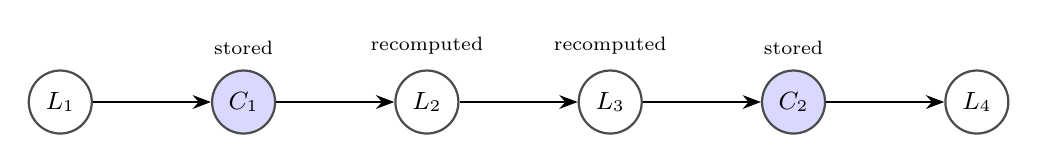
\begin{tikzpicture}[
    node distance=1.5cm, >=Stealth,
    layer/.style={circle, draw=black!70, thick, minimum size=0.8cm, font=\small},
    checkpoint/.style={circle, draw=black!70, thick, fill=blue!15,
                       minimum size=0.8cm, font=\small}
]
    \node[layer] (L1) {$L_1$};
    \node[checkpoint, right=of L1] (CP1) {$C_1$};
    \node[layer, right=of CP1] (L2) {$L_2$};
    \node[layer, right=of L2] (L3) {$L_3$};
    \node[checkpoint, right=of L3] (CP2) {$C_2$};
    \node[layer, right=of CP2] (L4) {$L_4$};
    \draw[-Stealth, thick] (L1) -- (CP1);
    \draw[-Stealth, thick] (CP1) -- (L2);
    \draw[-Stealth, thick] (L2) -- (L3);
    \draw[-Stealth, thick] (L3) -- (CP2);
    \draw[-Stealth, thick] (CP2) -- (L4);
    \node[above=2pt of CP1, font=\scriptsize] {stored};
    \node[above=2pt of L2, font=\scriptsize] {recomputed};
    \node[above=2pt of L3, font=\scriptsize] {recomputed};
    \node[above=2pt of CP2, font=\scriptsize] {stored};
\end{tikzpicture}
\end{center}

A subtle correctness issue arises for stochastic layers such as
\textbf{Dropout}. Recomputing the forward pass will, in general, draw a
\emph{different} random mask, yielding gradients that are inconsistent
with the loss they are meant to differentiate.

\begin{remark}
The remedy is not to store the activation tensor---which would defeat the
purpose---but to save the \emph{PRNG seed} at each checkpoint and restore
it during recomputation. Pseudo-randomness is cheap to reproduce exactly;
floating-point non-determinism arising from non-deterministic reduction
orderings on the GPU is another matter, and is typically tolerated in
practice for the sake of throughput.
\end{remark}

\subsection{Checkpointing Strategies}

\begin{enumerate}[leftmargin=1.8em, itemsep=2pt]
    \item \textbf{Single checkpoint.} One checkpoint at the input; all
    else is recomputed. Minimal memory, maximal compute overhead.
    \item \textbf{Multiple checkpoints.} Activations stored at several
    strategic layers.
    \item \textbf{Periodic (every $N$-th layer).} A simple heuristic that
    balances storage against rematerialisation cost.
    \item \textbf{Hierarchical / nested.} Checkpoints within checkpoints,
    e.g., one per Transformer block with further sub-checkpoints inside.
\end{enumerate}

The canonical reference is Chen et al.,
\href{https://arxiv.org/pdf/1604.06174.pdf}{arXiv:1604.06174}. For more details, see TensorFlow implementation
(\href{http://github.com/cybertronai/gradient-checkpointing}{\texttt{cybertronai/gradient-checkpointing}})
and to the PyTorch API,
\href{http://pytorch.org/docs/stable/checkpoint.html}{\texttt{torch.utils.checkpoint}}.

%%%%%%%%%%%%%%%%%%%%%%%%%%%%%%%%%%%%%%%%%%%%%%%%%%%%%%%%%%%%%%%%%%%%%%%%
\section{Memory Offloading}
%%%%%%%%%%%%%%%%%%%%%%%%%%%%%%%%%%%%%%%%%%%%%%%%%%%%%%%%%%%%%%%%%%%%%%%%

Checkpointing addresses \emph{activation} memory by trading compute for
storage. It does nothing for \emph{parameters}, \emph{gradients}, or
\emph{optimizer states}---quantities that accumulate information over
time and cannot be recomputed. For these we employ \emph{offloading}: the
relocation of data from high-bandwidth GPU memory (VRAM) to slower but
vastly larger CPU RAM (DRAM) or NVMe storage.


\begin{definition}
\textbf{Parameter-based memory} (parameters, gradients, optimizer states)
is allocated prior to processing any example and is independent of the
input. \textbf{Instance-dependent memory} (activations) scales with batch
size and sequence length.
\end{definition}


Offloading is not free. The GPU communicates with the host over the PCIe
bus, whose bandwidth is orders of magnitude less than the internal memory
bandwidth of the GPU. The training regime can thus shift from
compute-bound to transfer-bound.

\begin{center}
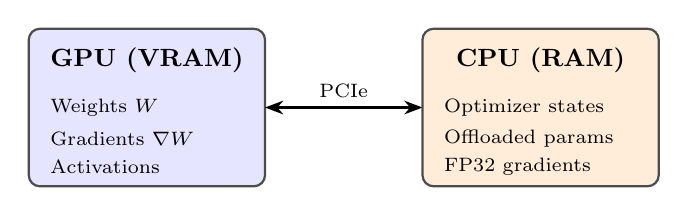
\begin{tikzpicture}[font=\small, >=Stealth]
    \draw[thick, draw=black!70, fill=blue!10, rounded corners] (0,0) rectangle (3,2);
    \node at (1.5, 1.6) {\textbf{GPU (VRAM)}};
    \node[anchor=west, font=\scriptsize] at (0.15, 1.0) {Weights $W$};
    \node[anchor=west, font=\scriptsize] at (0.15, 0.6) {Gradients $\grad W$};
    \node[anchor=west, font=\scriptsize] at (0.15, 0.25) {Activations};
    \draw[thick, <->] (3,1) -- (5,1) node[midway, above, font=\scriptsize] {PCIe};
    \draw[thick, draw=black!70, fill=orange!15, rounded corners] (5,0) rectangle (8,2);
    \node at (6.5, 1.6) {\textbf{CPU (RAM)}};
    \node[anchor=west, font=\scriptsize] at (5.15, 1.0) {Optimizer states};
    \node[anchor=west, font=\scriptsize] at (5.15, 0.6) {Offloaded params};
    \node[anchor=west, font=\scriptsize] at (5.15, 0.25) {FP32 gradients};
\end{tikzpicture}
\end{center}


The naive offloading loop---fetch a layer, compute, evict---is ruinous
during single-token LLM inference: gigabytes are shipped across PCIe for
a handful of FLOPs. An optimised pipeline, exemplified by
\href{https://arxiv.org/abs/2002.05645}{L2L execution}, proceeds as
follows:

\begin{enumerate}[leftmargin=1.8em, itemsep=2pt]
    \item All layers reside initially on the CPU.
    \item A contiguous block of $k$ layers is moved to the GPU.
    \item Layers are evicted only after their computation is complete.
    \item The $(k{+}1)$-th layer is pre-fetched asynchronously while the
    $k$-th is being processed---latency hiding by overlap.
\end{enumerate}

\begin{center}
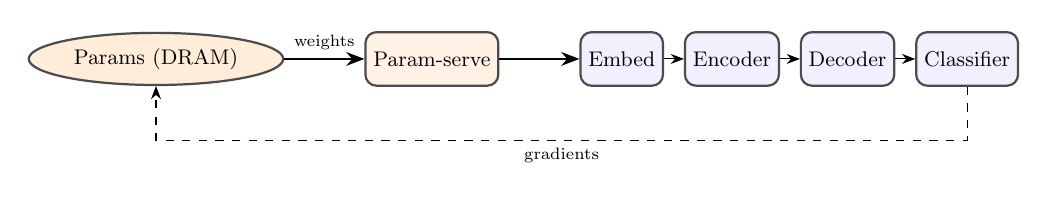
\begin{tikzpicture}[
    font=\small, >=Stealth, scale=0.85, transform shape,
    bx/.style={rectangle, rounded corners, draw=black!70, thick,
               fill=blue!6, minimum height=0.8cm}
]
    \node[ellipse, draw=black!70, thick, fill=orange!15, minimum width=3cm] (dram) {Params (DRAM)};
    \node[bx, fill=orange!10, right=1.2cm of dram] (host) {Param-serve};
    \node[bx, right=1.2cm of host] (embed) {Embed};
    \node[bx, right=0.3cm of embed] (enc) {Encoder};
    \node[bx, right=0.3cm of enc] (dec) {Decoder};
    \node[bx, right=0.3cm of dec] (cls) {Classifier};
    \draw[-Stealth, thick] (dram) -- node[above, font=\scriptsize] {weights} (host);
    \draw[-Stealth, thick] (host) -- (embed);
    \draw[-Stealth] (embed) -- (enc);
    \draw[-Stealth] (enc) -- (dec);
    \draw[-Stealth] (dec) -- (cls);
    \draw[-Stealth, dashed] (cls.south) -- ++(0,-0.8) -|
        node[pos=0.25, below, font=\scriptsize] {gradients} (dram.south);
\end{tikzpicture}
\end{center}

Empirically the overhead of offloading sits in the $20$--$50\%$ range, a
cost that can be amortised by larger effective batches.

\subsection{ZeRO-Offload}

The DeepSpeed framework's \textsc{ZeRO-Offload}
(\href{https://arxiv.org/abs/2101.06840}{arXiv:2101.06840}) refines this
idea by explicitly separating roles between devices:

\begin{itemize}[leftmargin=1.5em, itemsep=2pt]
    \item \textbf{Optimizer states.} Adam retains the first moment $m$
    and second moment $v$, each the size of the parameters. To preserve
    numerical stability, these are held in FP32 on the CPU---\emph{tripling}
    the effective parameter footprint.
    \item \textbf{Parameters.} FP16 on the GPU.
    \item \textbf{Gradients.} Computed in FP16 on the GPU, offloaded and
    accumulated in FP32 on the CPU.
\end{itemize}

The optimiser step proper,
\begin{equation}
\theta_{t+1} \;=\; \theta_t - \mathrm{Update}\!\left(\theta_t,
    \grad\theta_t, m_t, v_t\right),
\end{equation}
is performed on the CPU---feasible because it consists of element-wise
operations rather than matrix multiplications---with the updated
parameters swapped back to the GPU in time for the next forward pass. By
overlapping the \emph{computation stream} (GPU forward/backward) with a
separate \emph{swapping stream} (GPU$\leftrightarrow$CPU transfers), the
accelerator is rarely idle.

\begin{center}
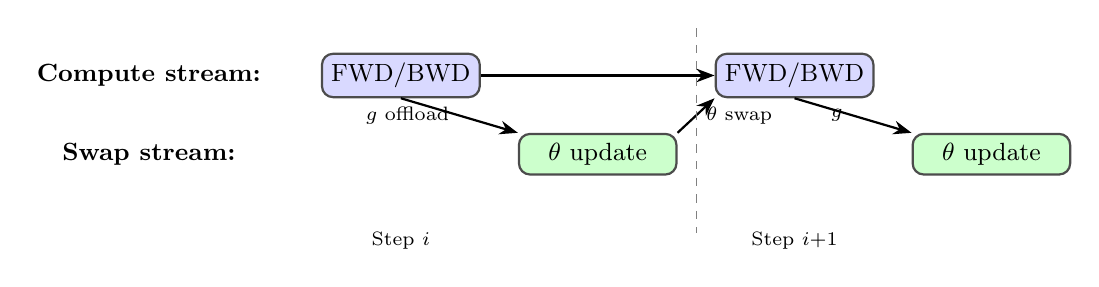
\begin{tikzpicture}[>=Stealth, font=\small]
    \node (compstream) at (-3.2, 1.5) {\textbf{Compute stream:}};
    \node (swapstream) at (-3.2, 0.5) {\textbf{Swap stream:}};
    \node[rectangle, rounded corners, draw=black!70, thick, fill=blue!15, minimum width=2cm] (g1) at (0, 1.5) {FWD/BWD};
    \node[rectangle, rounded corners, draw=black!70, thick, fill=green!20, minimum width=2cm] (c1) at (2.5, 0.5) {$\theta$ update};
    \node[rectangle, rounded corners, draw=black!70, thick, fill=blue!15, minimum width=2cm] (g2) at (5, 1.5) {FWD/BWD};
    \node[rectangle, rounded corners, draw=black!70, thick, fill=green!20, minimum width=2cm] (c2) at (7.5, 0.5) {$\theta$ update};
    \draw[-Stealth, thick] (g1) -- (g2);
    \draw[-Stealth, thick] (g1.south) -- node[midway, left, font=\scriptsize] {$g$ offload} (c1.north west);
    \draw[-Stealth, thick] (c1.north east) -- node[midway, right, font=\scriptsize] {$\theta$ swap} (g2.south west);
    \draw[-Stealth, thick] (g2.south) -- node[midway, left, font=\scriptsize] {$g$ } (c2.north west);
    \draw[dashed, black!50] (3.75, 2.1) -- (3.75, -0.5);
    \node[font=\scriptsize] at (0, -0.6) {Step $i$};
    \node[font=\scriptsize] at (5, -0.6) {Step $i{+}1$};
\end{tikzpicture}
\end{center}

%%%%%%%%%%%%%%%%%%%%%%%%%%%%%%%%%%%%%%%%%%%%%%%%%%%%%%%%%%%%%%%%%%%%%%%%
\section{Pipeline Parallelism}
%%%%%%%%%%%%%%%%%%%%%%%%%%%%%%%%%%%%%%%%%%%%%%%%%%%%%%%%%%%%%%%%%%%%%%%%

When even the parameters fail to fit on a single device, we must
\emph{partition the model itself} across GPUs. The simplest such strategy
is \emph{pipeline parallelism}: successive layers are assigned to
successive devices, and activations flow from one to the next.

All the schedule diagrams in this section follow one convention. Time
runs left to right and each row is a device. A blue box is a forward pass
and an orange box a backward pass, each labelled with the number of the
micro-batch it processes; a backward pass is drawn twice as long as a
forward pass, as it is in practice (it computes gradients with respect to
both activations and weights). Hatched regions are idle time---the
\emph{bubble}.

Cut the model into $N$ consecutive stages and put stage $k$ on device
$k$. One training step sends the batch forward through devices
$1,\ldots,N$, computes the loss on the last device, and sends the
gradients backward through devices $N,\ldots,1$.

\begin{center}
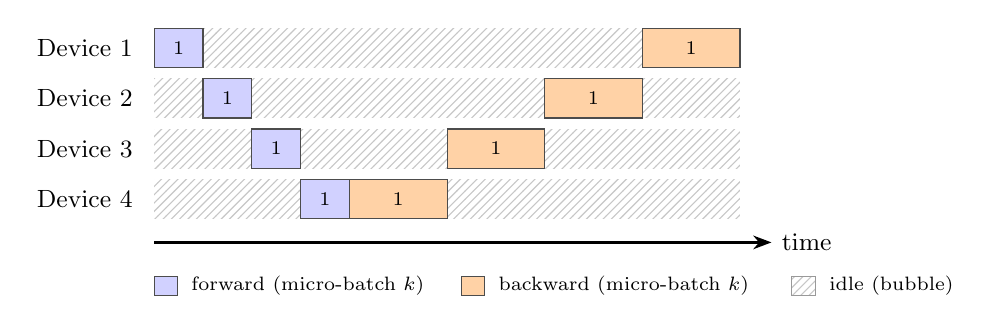
\begin{tikzpicture}[>=Stealth, font=\small]
\node[anchor=east] at (-0.15,-0.250) {Device 1};
\node[anchor=east] at (-0.15,-0.890) {Device 2};
\node[anchor=east] at (-0.15,-1.530) {Device 3};
\node[anchor=east] at (-0.15,-2.170) {Device 4};
\fill[pattern=north east lines, pattern color=black!22] (0.620,-0.500) rectangle (6.200,0.000);
\fill[pattern=north east lines, pattern color=black!22] (0.000,-1.140) rectangle (0.620,-0.640);
\fill[pattern=north east lines, pattern color=black!22] (1.240,-1.140) rectangle (4.960,-0.640);
\fill[pattern=north east lines, pattern color=black!22] (6.200,-1.140) rectangle (7.440,-0.640);
\fill[pattern=north east lines, pattern color=black!22] (0.000,-1.780) rectangle (1.240,-1.280);
\fill[pattern=north east lines, pattern color=black!22] (1.860,-1.780) rectangle (3.720,-1.280);
\fill[pattern=north east lines, pattern color=black!22] (4.960,-1.780) rectangle (7.440,-1.280);
\fill[pattern=north east lines, pattern color=black!22] (0.000,-2.420) rectangle (1.860,-1.920);
\fill[pattern=north east lines, pattern color=black!22] (3.720,-2.420) rectangle (7.440,-1.920);
\draw[fill=blue!18, draw=black!70, line width=0.4pt] (0.000,-0.500) rectangle (0.620,0.000);
\node[font=\scriptsize] at (0.310,-0.250) {1};
\draw[fill=orange!35, draw=black!70, line width=0.4pt] (6.200,-0.500) rectangle (7.440,0.000);
\node[font=\scriptsize] at (6.820,-0.250) {1};
\draw[fill=blue!18, draw=black!70, line width=0.4pt] (0.620,-1.140) rectangle (1.240,-0.640);
\node[font=\scriptsize] at (0.930,-0.890) {1};
\draw[fill=orange!35, draw=black!70, line width=0.4pt] (4.960,-1.140) rectangle (6.200,-0.640);
\node[font=\scriptsize] at (5.580,-0.890) {1};
\draw[fill=blue!18, draw=black!70, line width=0.4pt] (1.240,-1.780) rectangle (1.860,-1.280);
\node[font=\scriptsize] at (1.550,-1.530) {1};
\draw[fill=orange!35, draw=black!70, line width=0.4pt] (3.720,-1.780) rectangle (4.960,-1.280);
\node[font=\scriptsize] at (4.340,-1.530) {1};
\draw[fill=blue!18, draw=black!70, line width=0.4pt] (1.860,-2.420) rectangle (2.480,-1.920);
\node[font=\scriptsize] at (2.170,-2.170) {1};
\draw[fill=orange!35, draw=black!70, line width=0.4pt] (2.480,-2.420) rectangle (3.720,-1.920);
\node[font=\scriptsize] at (3.100,-2.170) {1};
\draw[-Stealth, thick] (0,-2.720) -- (7.840,-2.720) node[right, font=\small] {time};
\draw[fill=blue!18, draw=black!70, line width=0.4pt] (0,-3.390) rectangle (0.3,-3.150); \node[anchor=west, font=\scriptsize] at (0.35,-3.270) {forward (micro-batch $k$)};
\draw[fill=orange!35, draw=black!70, line width=0.4pt] (3.9,-3.390) rectangle (4.2,-3.150); \node[anchor=west, font=\scriptsize] at (4.25,-3.270) {backward (micro-batch $k$)};
\fill[pattern=north east lines, pattern color=black!22] (8.1,-3.390) rectangle (8.4,-3.150); \draw[black!40] (8.1,-3.390) rectangle (8.4,-3.150); \node[anchor=west, font=\scriptsize] at (8.45,-3.270) {idle (bubble)};

\end{tikzpicture}
\par\smallskip
{\small Naive pipeline, $N=4$ devices and a single batch in flight: at
any moment only one device is working.}
\end{center}

With a single batch in flight this scheme is sequential: device $i+1$
waits on device $i$. At every instant exactly one device works while the
other $N-1$ idle, so with $N=4$ each device is busy a quarter of the time
and $75\%$ of the hardware is wasted. The throughput is $\Theta(1)$ while
the model size scales as $\Theta(N)$ across $N$ devices---a single GPU's
worth of useful work, spread across a rack.

\subsection{GPipe: Micro-batching}

\textsc{GPipe} (\href{https://arxiv.org/abs/1811.06965}{Huang et al.,
2018}) resolves this by splitting the global batch into $m$
\emph{micro-batches}. Device $1$ processes micro-batch $1$, then
immediately begins micro-batch $2$ while device $2$ consumes the output of
micro-batch $1$, and so on---a true assembly line. Once every forward pass
has finished, the backward passes run through the micro-batches in
reverse order, and a single optimiser step is taken at the end.

\begin{center}
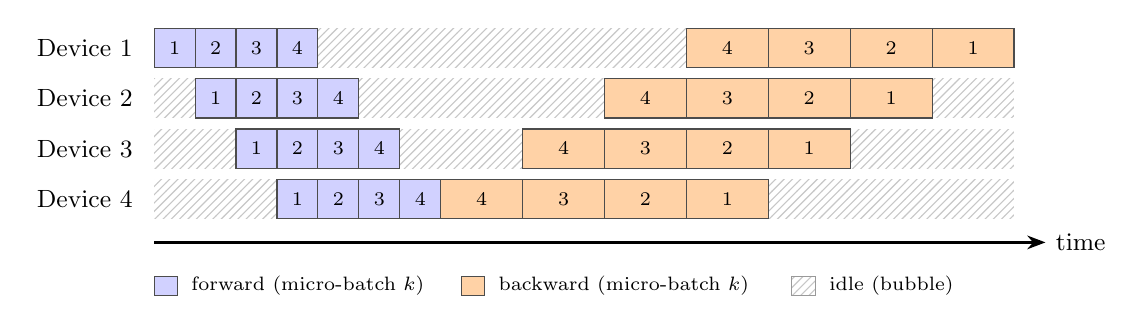
\begin{tikzpicture}[>=Stealth, font=\small]
\node[anchor=east] at (-0.15,-0.250) {Device 1};
\node[anchor=east] at (-0.15,-0.890) {Device 2};
\node[anchor=east] at (-0.15,-1.530) {Device 3};
\node[anchor=east] at (-0.15,-2.170) {Device 4};
\fill[pattern=north east lines, pattern color=black!22] (2.080,-0.500) rectangle (6.760,0.000);
\fill[pattern=north east lines, pattern color=black!22] (0.000,-1.140) rectangle (0.520,-0.640);
\fill[pattern=north east lines, pattern color=black!22] (2.600,-1.140) rectangle (5.720,-0.640);
\fill[pattern=north east lines, pattern color=black!22] (9.880,-1.140) rectangle (10.920,-0.640);
\fill[pattern=north east lines, pattern color=black!22] (0.000,-1.780) rectangle (1.040,-1.280);
\fill[pattern=north east lines, pattern color=black!22] (3.120,-1.780) rectangle (4.680,-1.280);
\fill[pattern=north east lines, pattern color=black!22] (8.840,-1.780) rectangle (10.920,-1.280);
\fill[pattern=north east lines, pattern color=black!22] (0.000,-2.420) rectangle (1.560,-1.920);
\fill[pattern=north east lines, pattern color=black!22] (7.800,-2.420) rectangle (10.920,-1.920);
\draw[fill=blue!18, draw=black!70, line width=0.4pt] (0.000,-0.500) rectangle (0.520,0.000);
\node[font=\scriptsize] at (0.260,-0.250) {1};
\draw[fill=blue!18, draw=black!70, line width=0.4pt] (0.520,-0.500) rectangle (1.040,0.000);
\node[font=\scriptsize] at (0.780,-0.250) {2};
\draw[fill=blue!18, draw=black!70, line width=0.4pt] (1.040,-0.500) rectangle (1.560,0.000);
\node[font=\scriptsize] at (1.300,-0.250) {3};
\draw[fill=blue!18, draw=black!70, line width=0.4pt] (1.560,-0.500) rectangle (2.080,0.000);
\node[font=\scriptsize] at (1.820,-0.250) {4};
\draw[fill=orange!35, draw=black!70, line width=0.4pt] (6.760,-0.500) rectangle (7.800,0.000);
\node[font=\scriptsize] at (7.280,-0.250) {4};
\draw[fill=orange!35, draw=black!70, line width=0.4pt] (7.800,-0.500) rectangle (8.840,0.000);
\node[font=\scriptsize] at (8.320,-0.250) {3};
\draw[fill=orange!35, draw=black!70, line width=0.4pt] (8.840,-0.500) rectangle (9.880,0.000);
\node[font=\scriptsize] at (9.360,-0.250) {2};
\draw[fill=orange!35, draw=black!70, line width=0.4pt] (9.880,-0.500) rectangle (10.920,0.000);
\node[font=\scriptsize] at (10.400,-0.250) {1};
\draw[fill=blue!18, draw=black!70, line width=0.4pt] (0.520,-1.140) rectangle (1.040,-0.640);
\node[font=\scriptsize] at (0.780,-0.890) {1};
\draw[fill=blue!18, draw=black!70, line width=0.4pt] (1.040,-1.140) rectangle (1.560,-0.640);
\node[font=\scriptsize] at (1.300,-0.890) {2};
\draw[fill=blue!18, draw=black!70, line width=0.4pt] (1.560,-1.140) rectangle (2.080,-0.640);
\node[font=\scriptsize] at (1.820,-0.890) {3};
\draw[fill=blue!18, draw=black!70, line width=0.4pt] (2.080,-1.140) rectangle (2.600,-0.640);
\node[font=\scriptsize] at (2.340,-0.890) {4};
\draw[fill=orange!35, draw=black!70, line width=0.4pt] (5.720,-1.140) rectangle (6.760,-0.640);
\node[font=\scriptsize] at (6.240,-0.890) {4};
\draw[fill=orange!35, draw=black!70, line width=0.4pt] (6.760,-1.140) rectangle (7.800,-0.640);
\node[font=\scriptsize] at (7.280,-0.890) {3};
\draw[fill=orange!35, draw=black!70, line width=0.4pt] (7.800,-1.140) rectangle (8.840,-0.640);
\node[font=\scriptsize] at (8.320,-0.890) {2};
\draw[fill=orange!35, draw=black!70, line width=0.4pt] (8.840,-1.140) rectangle (9.880,-0.640);
\node[font=\scriptsize] at (9.360,-0.890) {1};
\draw[fill=blue!18, draw=black!70, line width=0.4pt] (1.040,-1.780) rectangle (1.560,-1.280);
\node[font=\scriptsize] at (1.300,-1.530) {1};
\draw[fill=blue!18, draw=black!70, line width=0.4pt] (1.560,-1.780) rectangle (2.080,-1.280);
\node[font=\scriptsize] at (1.820,-1.530) {2};
\draw[fill=blue!18, draw=black!70, line width=0.4pt] (2.080,-1.780) rectangle (2.600,-1.280);
\node[font=\scriptsize] at (2.340,-1.530) {3};
\draw[fill=blue!18, draw=black!70, line width=0.4pt] (2.600,-1.780) rectangle (3.120,-1.280);
\node[font=\scriptsize] at (2.860,-1.530) {4};
\draw[fill=orange!35, draw=black!70, line width=0.4pt] (4.680,-1.780) rectangle (5.720,-1.280);
\node[font=\scriptsize] at (5.200,-1.530) {4};
\draw[fill=orange!35, draw=black!70, line width=0.4pt] (5.720,-1.780) rectangle (6.760,-1.280);
\node[font=\scriptsize] at (6.240,-1.530) {3};
\draw[fill=orange!35, draw=black!70, line width=0.4pt] (6.760,-1.780) rectangle (7.800,-1.280);
\node[font=\scriptsize] at (7.280,-1.530) {2};
\draw[fill=orange!35, draw=black!70, line width=0.4pt] (7.800,-1.780) rectangle (8.840,-1.280);
\node[font=\scriptsize] at (8.320,-1.530) {1};
\draw[fill=blue!18, draw=black!70, line width=0.4pt] (1.560,-2.420) rectangle (2.080,-1.920);
\node[font=\scriptsize] at (1.820,-2.170) {1};
\draw[fill=blue!18, draw=black!70, line width=0.4pt] (2.080,-2.420) rectangle (2.600,-1.920);
\node[font=\scriptsize] at (2.340,-2.170) {2};
\draw[fill=blue!18, draw=black!70, line width=0.4pt] (2.600,-2.420) rectangle (3.120,-1.920);
\node[font=\scriptsize] at (2.860,-2.170) {3};
\draw[fill=blue!18, draw=black!70, line width=0.4pt] (3.120,-2.420) rectangle (3.640,-1.920);
\node[font=\scriptsize] at (3.380,-2.170) {4};
\draw[fill=orange!35, draw=black!70, line width=0.4pt] (3.640,-2.420) rectangle (4.680,-1.920);
\node[font=\scriptsize] at (4.160,-2.170) {4};
\draw[fill=orange!35, draw=black!70, line width=0.4pt] (4.680,-2.420) rectangle (5.720,-1.920);
\node[font=\scriptsize] at (5.200,-2.170) {3};
\draw[fill=orange!35, draw=black!70, line width=0.4pt] (5.720,-2.420) rectangle (6.760,-1.920);
\node[font=\scriptsize] at (6.240,-2.170) {2};
\draw[fill=orange!35, draw=black!70, line width=0.4pt] (6.760,-2.420) rectangle (7.800,-1.920);
\node[font=\scriptsize] at (7.280,-2.170) {1};
\draw[-Stealth, thick] (0,-2.720) -- (11.320,-2.720) node[right, font=\small] {time};
\draw[fill=blue!18, draw=black!70, line width=0.4pt] (0,-3.390) rectangle (0.3,-3.150); \node[anchor=west, font=\scriptsize] at (0.35,-3.270) {forward (micro-batch $k$)};
\draw[fill=orange!35, draw=black!70, line width=0.4pt] (3.9,-3.390) rectangle (4.2,-3.150); \node[anchor=west, font=\scriptsize] at (4.25,-3.270) {backward (micro-batch $k$)};
\fill[pattern=north east lines, pattern color=black!22] (8.1,-3.390) rectangle (8.4,-3.150); \draw[black!40] (8.1,-3.390) rectangle (8.4,-3.150); \node[anchor=west, font=\scriptsize] at (8.45,-3.270) {idle (bubble)};

\end{tikzpicture}
\par\smallskip
{\small GPipe schedule, $N=4$ devices and $m=4$ micro-batches. The
hatched triangles at the start and at the end are the bubble.}
\end{center}

\begin{proposition}[Pipeline bubble]
\label{prop:bubble}
Assume that the stages are balanced, that communication between devices
is free, and that one micro-batch takes $f$ time units forward and $b$
backward on every device (in the figures $f=1$, $b=2$). With $N$ devices
and $m$ micro-batches, the fraction of the step that each device spends
idle is
\begin{equation}
\mathrm{bubble} = \frac{N-1}{m + N - 1},
\end{equation}
regardless of $f$ and $b$. It vanishes as $m \to \infty$.
\end{proposition}

\begin{proof}[Derivation]
The bubble is the idle share of the step, so we need two numbers: how long
a device \emph{works}, and how long the whole step \emph{lasts}.

\smallskip
\noindent\textbf{Step 1: useful time.} Every device processes all $m$
micro-batches, and each costs $f+b$:
\[
  T_{\mathrm{work}} = m\,(f+b).
\]

\noindent\textbf{Step 2: duration of the step.} Follow the last device,
because it finishes the forward phase last and sits on the critical path.
\begin{enumerate}[label=(\alph*), leftmargin=1.8em, itemsep=2pt]
    \item \emph{Fill.} Device $N$ cannot start until micro-batch $1$ has
    passed through the $N-1$ earlier stages, so it idles for $(N-1)f$.
    \item \emph{Steady work.} From then on it never waits: it runs the $m$
    forward passes back to back and then, since the loss is computed on
    this very device, immediately the $m$ backward passes. This takes
    $m(f+b)$.
    \item \emph{Drain.} Backward passes run in reverse order, so
    micro-batch $1$ is the last one. When device $N$ finishes it, its
    gradient still has to travel through devices $N-1,\ldots,1$, spending
    $b$ on each: $(N-1)b$.
\end{enumerate}
Adding up,
\[
  T = (N-1)f + m(f+b) + (N-1)b = (m+N-1)(f+b).
\]

\noindent\textbf{Step 3: idle fraction.} Each device is busy for
$T_{\mathrm{work}}$ out of $T$, so it idles for
\[
  T - T_{\mathrm{work}} = (N-1)(f+b),
  \qquad
  \mathrm{bubble} = \frac{T - T_{\mathrm{work}}}{T}
  = \frac{(N-1)(f+b)}{(m+N-1)(f+b)} = \frac{N-1}{m+N-1}.
\]
The factor $f+b$ cancels, which is why the answer does not depend on the
ratio of forward to backward cost.
\end{proof}

The idle time per device, $(N-1)(f+b)$, is a \emph{fixed} cost that does not
depend on $m$, while the useful work $m(f+b)$ grows linearly with $m$. This
is why more micro-batches shrink the bubble. For $m=1$ the formula gives
$\tfrac{N-1}{N}$, which is exactly the naive pipeline above: with $N=4$, a
fraction $75\%$ of the time is wasted.

Micro-batching is not free: the activations of all $m$ micro-batches stay
alive until their backward passes begin, so peak activation memory grows
with $m$ (the GPipe paper combines the schedule with activation
checkpointing for exactly this reason).

\subsection{1F1B: One-Forward-One-Backward}

A more sophisticated schedule, \emph{1F1B}, interleaves forward and
backward passes. Device $k$ (counting from $1$) first runs $N-k$ warm-up
forward passes; from then on it alternates: one forward on a fresh
micro-batch, one backward on the oldest one still outstanding. The last
device has no warm-up and starts alternating immediately.

\begin{center}
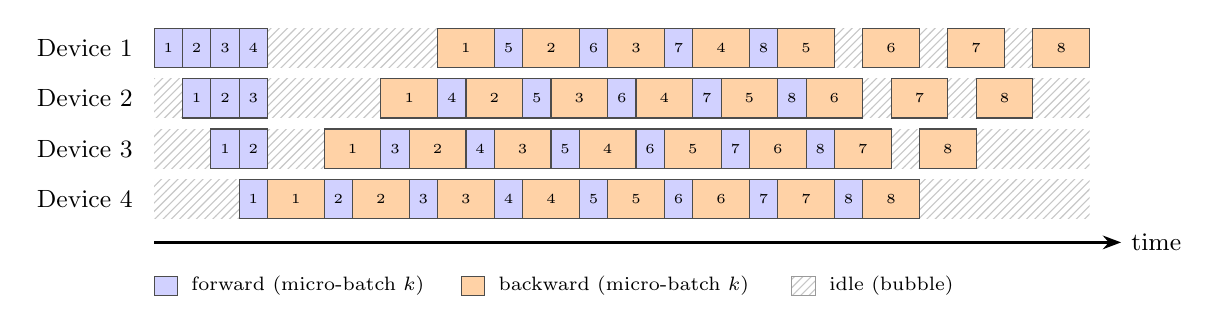
\begin{tikzpicture}[>=Stealth, font=\small]
\node[anchor=east] at (-0.15,-0.250) {Device 1};
\node[anchor=east] at (-0.15,-0.890) {Device 2};
\node[anchor=east] at (-0.15,-1.530) {Device 3};
\node[anchor=east] at (-0.15,-2.170) {Device 4};
\fill[pattern=north east lines, pattern color=black!22] (1.440,-0.500) rectangle (3.600,0.000);
\fill[pattern=north east lines, pattern color=black!22] (8.640,-0.500) rectangle (9.000,0.000);
\fill[pattern=north east lines, pattern color=black!22] (9.720,-0.500) rectangle (10.080,0.000);
\fill[pattern=north east lines, pattern color=black!22] (10.800,-0.500) rectangle (11.160,0.000);
\fill[pattern=north east lines, pattern color=black!22] (0.000,-1.140) rectangle (0.360,-0.640);
\fill[pattern=north east lines, pattern color=black!22] (1.440,-1.140) rectangle (2.880,-0.640);
\fill[pattern=north east lines, pattern color=black!22] (9.000,-1.140) rectangle (9.360,-0.640);
\fill[pattern=north east lines, pattern color=black!22] (10.080,-1.140) rectangle (10.440,-0.640);
\fill[pattern=north east lines, pattern color=black!22] (11.160,-1.140) rectangle (11.880,-0.640);
\fill[pattern=north east lines, pattern color=black!22] (0.000,-1.780) rectangle (0.720,-1.280);
\fill[pattern=north east lines, pattern color=black!22] (1.440,-1.780) rectangle (2.160,-1.280);
\fill[pattern=north east lines, pattern color=black!22] (9.360,-1.780) rectangle (9.720,-1.280);
\fill[pattern=north east lines, pattern color=black!22] (10.440,-1.780) rectangle (11.880,-1.280);
\fill[pattern=north east lines, pattern color=black!22] (0.000,-2.420) rectangle (1.080,-1.920);
\fill[pattern=north east lines, pattern color=black!22] (9.720,-2.420) rectangle (11.880,-1.920);
\draw[fill=blue!18, draw=black!70, line width=0.4pt] (0.000,-0.500) rectangle (0.360,0.000);
\node[font=\tiny] at (0.180,-0.250) {1};
\draw[fill=blue!18, draw=black!70, line width=0.4pt] (0.360,-0.500) rectangle (0.720,0.000);
\node[font=\tiny] at (0.540,-0.250) {2};
\draw[fill=blue!18, draw=black!70, line width=0.4pt] (0.720,-0.500) rectangle (1.080,0.000);
\node[font=\tiny] at (0.900,-0.250) {3};
\draw[fill=blue!18, draw=black!70, line width=0.4pt] (1.080,-0.500) rectangle (1.440,0.000);
\node[font=\tiny] at (1.260,-0.250) {4};
\draw[fill=orange!35, draw=black!70, line width=0.4pt] (3.600,-0.500) rectangle (4.320,0.000);
\node[font=\tiny] at (3.960,-0.250) {1};
\draw[fill=blue!18, draw=black!70, line width=0.4pt] (4.320,-0.500) rectangle (4.680,0.000);
\node[font=\tiny] at (4.500,-0.250) {5};
\draw[fill=orange!35, draw=black!70, line width=0.4pt] (4.680,-0.500) rectangle (5.400,0.000);
\node[font=\tiny] at (5.040,-0.250) {2};
\draw[fill=blue!18, draw=black!70, line width=0.4pt] (5.400,-0.500) rectangle (5.760,0.000);
\node[font=\tiny] at (5.580,-0.250) {6};
\draw[fill=orange!35, draw=black!70, line width=0.4pt] (5.760,-0.500) rectangle (6.480,0.000);
\node[font=\tiny] at (6.120,-0.250) {3};
\draw[fill=blue!18, draw=black!70, line width=0.4pt] (6.480,-0.500) rectangle (6.840,0.000);
\node[font=\tiny] at (6.660,-0.250) {7};
\draw[fill=orange!35, draw=black!70, line width=0.4pt] (6.840,-0.500) rectangle (7.560,0.000);
\node[font=\tiny] at (7.200,-0.250) {4};
\draw[fill=blue!18, draw=black!70, line width=0.4pt] (7.560,-0.500) rectangle (7.920,0.000);
\node[font=\tiny] at (7.740,-0.250) {8};
\draw[fill=orange!35, draw=black!70, line width=0.4pt] (7.920,-0.500) rectangle (8.640,0.000);
\node[font=\tiny] at (8.280,-0.250) {5};
\draw[fill=orange!35, draw=black!70, line width=0.4pt] (9.000,-0.500) rectangle (9.720,0.000);
\node[font=\tiny] at (9.360,-0.250) {6};
\draw[fill=orange!35, draw=black!70, line width=0.4pt] (10.080,-0.500) rectangle (10.800,0.000);
\node[font=\tiny] at (10.440,-0.250) {7};
\draw[fill=orange!35, draw=black!70, line width=0.4pt] (11.160,-0.500) rectangle (11.880,0.000);
\node[font=\tiny] at (11.520,-0.250) {8};
\draw[fill=blue!18, draw=black!70, line width=0.4pt] (0.360,-1.140) rectangle (0.720,-0.640);
\node[font=\tiny] at (0.540,-0.890) {1};
\draw[fill=blue!18, draw=black!70, line width=0.4pt] (0.720,-1.140) rectangle (1.080,-0.640);
\node[font=\tiny] at (0.900,-0.890) {2};
\draw[fill=blue!18, draw=black!70, line width=0.4pt] (1.080,-1.140) rectangle (1.440,-0.640);
\node[font=\tiny] at (1.260,-0.890) {3};
\draw[fill=orange!35, draw=black!70, line width=0.4pt] (2.880,-1.140) rectangle (3.600,-0.640);
\node[font=\tiny] at (3.240,-0.890) {1};
\draw[fill=blue!18, draw=black!70, line width=0.4pt] (3.600,-1.140) rectangle (3.960,-0.640);
\node[font=\tiny] at (3.780,-0.890) {4};
\draw[fill=orange!35, draw=black!70, line width=0.4pt] (3.960,-1.140) rectangle (4.680,-0.640);
\node[font=\tiny] at (4.320,-0.890) {2};
\draw[fill=blue!18, draw=black!70, line width=0.4pt] (4.680,-1.140) rectangle (5.040,-0.640);
\node[font=\tiny] at (4.860,-0.890) {5};
\draw[fill=orange!35, draw=black!70, line width=0.4pt] (5.040,-1.140) rectangle (5.760,-0.640);
\node[font=\tiny] at (5.400,-0.890) {3};
\draw[fill=blue!18, draw=black!70, line width=0.4pt] (5.760,-1.140) rectangle (6.120,-0.640);
\node[font=\tiny] at (5.940,-0.890) {6};
\draw[fill=orange!35, draw=black!70, line width=0.4pt] (6.120,-1.140) rectangle (6.840,-0.640);
\node[font=\tiny] at (6.480,-0.890) {4};
\draw[fill=blue!18, draw=black!70, line width=0.4pt] (6.840,-1.140) rectangle (7.200,-0.640);
\node[font=\tiny] at (7.020,-0.890) {7};
\draw[fill=orange!35, draw=black!70, line width=0.4pt] (7.200,-1.140) rectangle (7.920,-0.640);
\node[font=\tiny] at (7.560,-0.890) {5};
\draw[fill=blue!18, draw=black!70, line width=0.4pt] (7.920,-1.140) rectangle (8.280,-0.640);
\node[font=\tiny] at (8.100,-0.890) {8};
\draw[fill=orange!35, draw=black!70, line width=0.4pt] (8.280,-1.140) rectangle (9.000,-0.640);
\node[font=\tiny] at (8.640,-0.890) {6};
\draw[fill=orange!35, draw=black!70, line width=0.4pt] (9.360,-1.140) rectangle (10.080,-0.640);
\node[font=\tiny] at (9.720,-0.890) {7};
\draw[fill=orange!35, draw=black!70, line width=0.4pt] (10.440,-1.140) rectangle (11.160,-0.640);
\node[font=\tiny] at (10.800,-0.890) {8};
\draw[fill=blue!18, draw=black!70, line width=0.4pt] (0.720,-1.780) rectangle (1.080,-1.280);
\node[font=\tiny] at (0.900,-1.530) {1};
\draw[fill=blue!18, draw=black!70, line width=0.4pt] (1.080,-1.780) rectangle (1.440,-1.280);
\node[font=\tiny] at (1.260,-1.530) {2};
\draw[fill=orange!35, draw=black!70, line width=0.4pt] (2.160,-1.780) rectangle (2.880,-1.280);
\node[font=\tiny] at (2.520,-1.530) {1};
\draw[fill=blue!18, draw=black!70, line width=0.4pt] (2.880,-1.780) rectangle (3.240,-1.280);
\node[font=\tiny] at (3.060,-1.530) {3};
\draw[fill=orange!35, draw=black!70, line width=0.4pt] (3.240,-1.780) rectangle (3.960,-1.280);
\node[font=\tiny] at (3.600,-1.530) {2};
\draw[fill=blue!18, draw=black!70, line width=0.4pt] (3.960,-1.780) rectangle (4.320,-1.280);
\node[font=\tiny] at (4.140,-1.530) {4};
\draw[fill=orange!35, draw=black!70, line width=0.4pt] (4.320,-1.780) rectangle (5.040,-1.280);
\node[font=\tiny] at (4.680,-1.530) {3};
\draw[fill=blue!18, draw=black!70, line width=0.4pt] (5.040,-1.780) rectangle (5.400,-1.280);
\node[font=\tiny] at (5.220,-1.530) {5};
\draw[fill=orange!35, draw=black!70, line width=0.4pt] (5.400,-1.780) rectangle (6.120,-1.280);
\node[font=\tiny] at (5.760,-1.530) {4};
\draw[fill=blue!18, draw=black!70, line width=0.4pt] (6.120,-1.780) rectangle (6.480,-1.280);
\node[font=\tiny] at (6.300,-1.530) {6};
\draw[fill=orange!35, draw=black!70, line width=0.4pt] (6.480,-1.780) rectangle (7.200,-1.280);
\node[font=\tiny] at (6.840,-1.530) {5};
\draw[fill=blue!18, draw=black!70, line width=0.4pt] (7.200,-1.780) rectangle (7.560,-1.280);
\node[font=\tiny] at (7.380,-1.530) {7};
\draw[fill=orange!35, draw=black!70, line width=0.4pt] (7.560,-1.780) rectangle (8.280,-1.280);
\node[font=\tiny] at (7.920,-1.530) {6};
\draw[fill=blue!18, draw=black!70, line width=0.4pt] (8.280,-1.780) rectangle (8.640,-1.280);
\node[font=\tiny] at (8.460,-1.530) {8};
\draw[fill=orange!35, draw=black!70, line width=0.4pt] (8.640,-1.780) rectangle (9.360,-1.280);
\node[font=\tiny] at (9.000,-1.530) {7};
\draw[fill=orange!35, draw=black!70, line width=0.4pt] (9.720,-1.780) rectangle (10.440,-1.280);
\node[font=\tiny] at (10.080,-1.530) {8};
\draw[fill=blue!18, draw=black!70, line width=0.4pt] (1.080,-2.420) rectangle (1.440,-1.920);
\node[font=\tiny] at (1.260,-2.170) {1};
\draw[fill=orange!35, draw=black!70, line width=0.4pt] (1.440,-2.420) rectangle (2.160,-1.920);
\node[font=\tiny] at (1.800,-2.170) {1};
\draw[fill=blue!18, draw=black!70, line width=0.4pt] (2.160,-2.420) rectangle (2.520,-1.920);
\node[font=\tiny] at (2.340,-2.170) {2};
\draw[fill=orange!35, draw=black!70, line width=0.4pt] (2.520,-2.420) rectangle (3.240,-1.920);
\node[font=\tiny] at (2.880,-2.170) {2};
\draw[fill=blue!18, draw=black!70, line width=0.4pt] (3.240,-2.420) rectangle (3.600,-1.920);
\node[font=\tiny] at (3.420,-2.170) {3};
\draw[fill=orange!35, draw=black!70, line width=0.4pt] (3.600,-2.420) rectangle (4.320,-1.920);
\node[font=\tiny] at (3.960,-2.170) {3};
\draw[fill=blue!18, draw=black!70, line width=0.4pt] (4.320,-2.420) rectangle (4.680,-1.920);
\node[font=\tiny] at (4.500,-2.170) {4};
\draw[fill=orange!35, draw=black!70, line width=0.4pt] (4.680,-2.420) rectangle (5.400,-1.920);
\node[font=\tiny] at (5.040,-2.170) {4};
\draw[fill=blue!18, draw=black!70, line width=0.4pt] (5.400,-2.420) rectangle (5.760,-1.920);
\node[font=\tiny] at (5.580,-2.170) {5};
\draw[fill=orange!35, draw=black!70, line width=0.4pt] (5.760,-2.420) rectangle (6.480,-1.920);
\node[font=\tiny] at (6.120,-2.170) {5};
\draw[fill=blue!18, draw=black!70, line width=0.4pt] (6.480,-2.420) rectangle (6.840,-1.920);
\node[font=\tiny] at (6.660,-2.170) {6};
\draw[fill=orange!35, draw=black!70, line width=0.4pt] (6.840,-2.420) rectangle (7.560,-1.920);
\node[font=\tiny] at (7.200,-2.170) {6};
\draw[fill=blue!18, draw=black!70, line width=0.4pt] (7.560,-2.420) rectangle (7.920,-1.920);
\node[font=\tiny] at (7.740,-2.170) {7};
\draw[fill=orange!35, draw=black!70, line width=0.4pt] (7.920,-2.420) rectangle (8.640,-1.920);
\node[font=\tiny] at (8.280,-2.170) {7};
\draw[fill=blue!18, draw=black!70, line width=0.4pt] (8.640,-2.420) rectangle (9.000,-1.920);
\node[font=\tiny] at (8.820,-2.170) {8};
\draw[fill=orange!35, draw=black!70, line width=0.4pt] (9.000,-2.420) rectangle (9.720,-1.920);
\node[font=\tiny] at (9.360,-2.170) {8};
\draw[-Stealth, thick] (0,-2.720) -- (12.280,-2.720) node[right, font=\small] {time};
\draw[fill=blue!18, draw=black!70, line width=0.4pt] (0,-3.390) rectangle (0.3,-3.150); \node[anchor=west, font=\scriptsize] at (0.35,-3.270) {forward (micro-batch $k$)};
\draw[fill=orange!35, draw=black!70, line width=0.4pt] (3.9,-3.390) rectangle (4.2,-3.150); \node[anchor=west, font=\scriptsize] at (4.25,-3.270) {backward (micro-batch $k$)};
\fill[pattern=north east lines, pattern color=black!22] (8.1,-3.390) rectangle (8.4,-3.150); \draw[black!40] (8.1,-3.390) rectangle (8.4,-3.150); \node[anchor=west, font=\scriptsize] at (8.45,-3.270) {idle (bubble)};

\end{tikzpicture}
\par\smallskip
{\small 1F1B schedule with a flush at the end of the batch, $N=4$ devices
and $m=8$ micro-batches.}
\end{center}

Two things are worth noticing in the figure. First, the total time is the
same as in GPipe, $(m+N-1)\cdot 3 = 33$ units, and so is the bubble,
$\tfrac{N-1}{m+N-1}$: \emph{1F1B does not shrink the bubble}. Second, it
changes the memory profile. Because a device starts a backward pass as
soon as one is available, device $k$ never holds the activations of more
than $N-k+1$ micro-batches (at most $N$ on the first device), no matter
how large $m$ is; under GPipe all $m$ are alive at the peak. The memory
saved lets one afford a larger $m$, and hence a smaller bubble. This is the 1F1B
pipeline from Megatron-LM
(\href{https://arxiv.org/abs/2104.04473}{arXiv:2104.04473}).

\subsection{Reducing the Bubble Further: Split Backward Pass}

The backward pass of a fully connected layer naturally decomposes into
two independent operations:
\begin{align}
\grad_{\text{input}} \LL &: \text{needed by the previous stage;} \\
\grad_{\text{weight}} \LL &: \text{needed only by the optimiser step.}
\end{align}
In the standard schedule they are computed together, but the second is
not on the critical path of backpropagation. \emph{Zero-Bubble} schedules
(ZB1P, ZB-H1, ZB-H2---see
\href{https://arxiv.org/abs/2401.10241}{arXiv:2401.10241}) schedule the
weight-gradient computation opportunistically, collapsing the pipeline
bubble to nearly zero. A further refinement is described by DeepSeek
(\href{https://arxiv.org/abs/2412.19437}{arXiv:2412.19437}).

\subsection{When to Pipeline}

\begin{remark}
Pipelining is appropriate when \textbf{(i)} the model's parameters alone
exceed a single GPU's capacity and \textbf{(ii)} multiple GPUs are
available. It is \emph{not} the correct remedy for merely oversized
activations: use gradient checkpointing. It is not available with a
single GPU: use offloading. And it is rarely used alone---in production,
pipeline parallelism is combined with data parallelism, tensor
parallelism, and checkpointing to exploit every axis of hardware
structure.
\end{remark}

Practical implementations:
\begin{itemize}[leftmargin=1.5em, itemsep=2pt]
    \item a basic GPipe implementation:
          \href{https://github.com/kakaobrain/torchgpipe}{\texttt{torchgpipe}};
    \item the PyTorch built-in, covered in the official
          \href{https://pytorch.org/tutorials/intermediate/pipelining_tutorial.html}{pipelining
          tutorial};
    \item DeepSpeed's
          \href{https://deepspeed.readthedocs.io/en/latest/pipeline.html}{pipeline
          engine};
    \item custom pipelines in many applications, such as
          \href{https://github.com/NVIDIA/Megatron-LM}{Megatron-LM}
          (transformer-specific) and
          \href{https://github.com/databricks/megablocks}{Megablocks}
          (mixture-of-experts).
\end{itemize}

PyTorch provides pipeline primitives in
\texttt{torch.distributed.pipelining}:
\begin{lstlisting}
from torch.distributed.pipelining import ScheduleGPipe
schedule = ScheduleGPipe(stage, n_microbatches)
\end{lstlisting}

For hands-on practice, see a
\href{https://tinyurl.com/pytorch-pipelining}{simple pipelining tutorial
in PyTorch} and a tutorial on
\href{http://tinyurl.com/torch-rpc}{distributed model parallelism with
torch RPC}.

%%%%%%%%%%%%%%%%%%%%%%%%%%%%%%%%%%%%%%%%%%%%%%%%%%%%%%%%%%%%%%%%%%%%%%%%
\section{Tensor Parallelism}
\label{sec:tp}
%%%%%%%%%%%%%%%%%%%%%%%%%%%%%%%%%%%%%%%%%%%%%%%%%%%%%%%%%%%%%%%%%%%%%%%%

Where pipeline parallelism partitions \emph{across layers}, tensor
parallelism partitions \emph{within a single layer}. The idea is older
than its name: AlexNet
(\href{https://papers.nips.cc/paper/4824-imagenet-classification-with-deep-convolutional-neural-networks}{2012})
already split a convolutional network's channels between two GPUs,
synchronising only at select interfaces; combining such model parallelism
with data parallelism is discussed in
\href{https://arxiv.org/abs/1404.5997}{arXiv:1404.5997}.

The whole section rests on a single question: \emph{a layer is a matrix
product $Y=XW$; how can several GPUs each compute a piece of it?} There
are exactly two natural ways to cut the weight matrix, and everything
else---the Transformer recipe, the communication pattern, the cost---is a
consequence of how they combine.


Let $X\in\mathbb{R}^{n\times d}$ hold $n$ tokens with $d$ features each,
let $W\in\mathbb{R}^{d\times m}$ be a weight matrix, and let two GPUs
share the work (the same ideas hold for any number $k$ of GPUs).

\paragraph{Cut 1: column-parallel.}
Split $W$ into blocks of \emph{columns}, $W=[A_1\;A_2]$. Each GPU needs the
\emph{whole} input $X$, multiplies it by its own block, and produces its own
\emph{columns} of the output. Nothing has to be added together, because
different GPUs produce different output entries:
\[
  Y \;=\; XW \;=\; \bigl[\,XA_1 \;\;\; XA_2\,\bigr] \;=\; [\,Y_1\;\;Y_2\,].
\]

\begin{center}
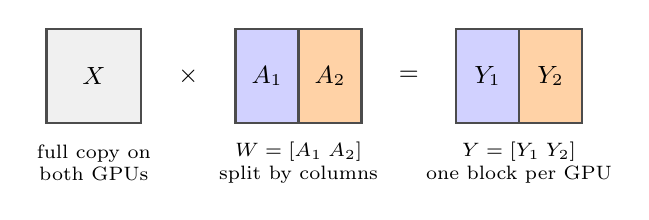
\begin{tikzpicture}[font=\small]
  % X replicated
  \draw[fill=gray!12, draw=black!70, thick] (0,0) rectangle (1.2,1.2);
  \node at (0.6,0.6) {$X$};
  \node[font=\scriptsize, align=center] at (0.6,-0.5) {full copy on\\both GPUs};
  \node at (1.8,0.6) {$\times$};
  % W blocks
  \draw[fill=blue!18, draw=black!70, thick] (2.4,0) rectangle (3.2,1.2);
  \draw[fill=orange!35, draw=black!70, thick] (3.2,0) rectangle (4.0,1.2);
  \node at (2.8,0.6) {$A_1$}; \node at (3.6,0.6) {$A_2$};
  \node[font=\scriptsize, align=center] at (3.2,-0.5) {$W=[A_1\;A_2]$\\split by columns};
  \node at (4.6,0.6) {$=$};
  % Y blocks
  \draw[fill=blue!18, draw=black!70, thick] (5.2,0) rectangle (6.0,1.2);
  \draw[fill=orange!35, draw=black!70, thick] (6.0,0) rectangle (6.8,1.2);
  \node at (5.6,0.6) {$Y_1$}; \node at (6.4,0.6) {$Y_2$};
  \node[font=\scriptsize, align=center] at (6.0,-0.5) {$Y=[Y_1\;Y_2]$\\one block per GPU};
\end{tikzpicture}
\end{center}

\paragraph{Cut 2: row-parallel.}
Split $W$ into blocks of \emph{rows}, $W=\bigl[\begin{smallmatrix}B_1\\
B_2\end{smallmatrix}\bigr]$. Now each GPU needs only the matching
\emph{columns} of the input, $X=[X_1\;X_2]$, because a block of rows of $W$
only ever touches the corresponding features of $X$. Each GPU produces a
full-size but \emph{incomplete} output---a partial sum---and the true
output is their sum:
\[
  Y \;=\; XW \;=\; X_1 B_1 \;+\; X_2 B_2 \;=\; P_1 + P_2 .
\]
The sum is a communication step: an \textsc{AllReduce}.

\begin{center}
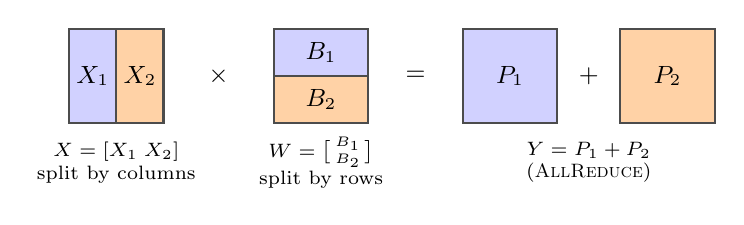
\begin{tikzpicture}[font=\small]
  % X split by columns
  \draw[fill=blue!18, draw=black!70, thick] (0,0) rectangle (0.6,1.2);
  \draw[fill=orange!35, draw=black!70, thick] (0.6,0) rectangle (1.2,1.2);
  \node at (0.3,0.6) {$X_1$}; \node at (0.9,0.6) {$X_2$};
  \node[font=\scriptsize, align=center] at (0.6,-0.5) {$X=[X_1\;X_2]$\\split by columns};
  \node at (1.9,0.6) {$\times$};
  % W split by rows
  \draw[fill=blue!18, draw=black!70, thick] (2.6,0.6) rectangle (3.8,1.2);
  \draw[fill=orange!35, draw=black!70, thick] (2.6,0) rectangle (3.8,0.6);
  \node at (3.2,0.9) {$B_1$}; \node at (3.2,0.3) {$B_2$};
  \node[font=\scriptsize, align=center] at (3.2,-0.5) {$W=\bigl[\begin{smallmatrix}B_1\\B_2\end{smallmatrix}\bigr]$\\split by rows};
  \node at (4.4,0.6) {$=$};
  % Partial outputs
  \draw[fill=blue!18, draw=black!70, thick] (5.0,0) rectangle (6.2,1.2);
  \node at (5.6,0.6) {$P_1$};
  \node at (6.6,0.6) {$+$};
  \draw[fill=orange!35, draw=black!70, thick] (7.0,0) rectangle (8.2,1.2);
  \node at (7.6,0.6) {$P_2$};
  \node[font=\scriptsize, align=center] at (6.6,-0.5) {$Y=P_1+P_2$\\(\textsc{AllReduce})};
\end{tikzpicture}
\end{center}

The rule of thumb to remember: \textbf{column-parallel needs the full
input and produces a sharded output with no communication; row-parallel
takes a sharded input and produces partial sums that must be added.}

\subsection{Why the Two Cuts Are Used Together}

Chaining two layers with a nonlinearity in between, $Y=\sigma(XW_1)\,W_2$
as in a Transformer MLP, one might ask which cut to use for which layer.
The answer is dictated by the nonlinearity $\sigma$.

\begin{example}[Why $W_1$ must be cut by columns]
\label{ex:tp-relu}
Suppose we cut $W_1$ by \emph{rows} instead. Then each GPU holds only a
partial sum $Z_1$ or $Z_2$ of every pre-activation $Z=Z_1+Z_2$. Consider a
single entry with $Z_1=1$ and $Z_2=-1$. The correct activation is
$\ReLU(Z_1+Z_2)=\ReLU(0)=0$. If each GPU applies the nonlinearity to its
own partial sum, adding the results gives $\ReLU(1)+\ReLU(-1)=1\neq0$.
The same failure occurs for $\GeLU$ or any nonlinear $\sigma$: in general
$\sigma(Z_1+Z_2)\neq\sigma(Z_1)+\sigma(Z_2)$. One would have to
\textsc{AllReduce} the pre-activations \emph{before} applying $\sigma$,
which costs an extra collective.

With a \emph{column} cut, each GPU owns complete pre-activation entries
(whole columns of $Z$), so it can apply $\sigma$ locally and correctly.
That is why the first layer is column-parallel. Its output is then
sharded by columns, which is exactly the sharded-by-columns input that the
row-parallel cut of the second layer wants---so the two layers connect
with no communication in between.
\end{example}

Putting it together for an MLP with hidden width $d_{ff}$ on two GPUs,
write $W_1=[A_1\;A_2]$ (column cut, $A_i\in\mathbb{R}^{d\times d_{ff}/2}$)
and $W_2=\bigl[\begin{smallmatrix}B_1\\B_2\end{smallmatrix}\bigr]$ (row
cut, $B_i\in\mathbb{R}^{d_{ff}/2\times d}$). GPU $i$ computes
\[
  Z_i=\GeLU(XA_i)\in\mathbb{R}^{n\times d_{ff}/2},\qquad
  P_i=Z_iB_i\in\mathbb{R}^{n\times d},\qquad
  Y=P_1+P_2 .
\]
Here is the whole block, with the two communication operators of the
Megatron-LM formulation marked $f$ and $g$: $f$ is the identity in the
forward pass and an \textsc{AllReduce} in the backward pass, and $g$ is an
\textsc{AllReduce} in the forward pass and the identity in the backward pass.
Over a forward and a backward pass the block therefore costs exactly two
\textsc{AllReduce} calls.

\begin{center}
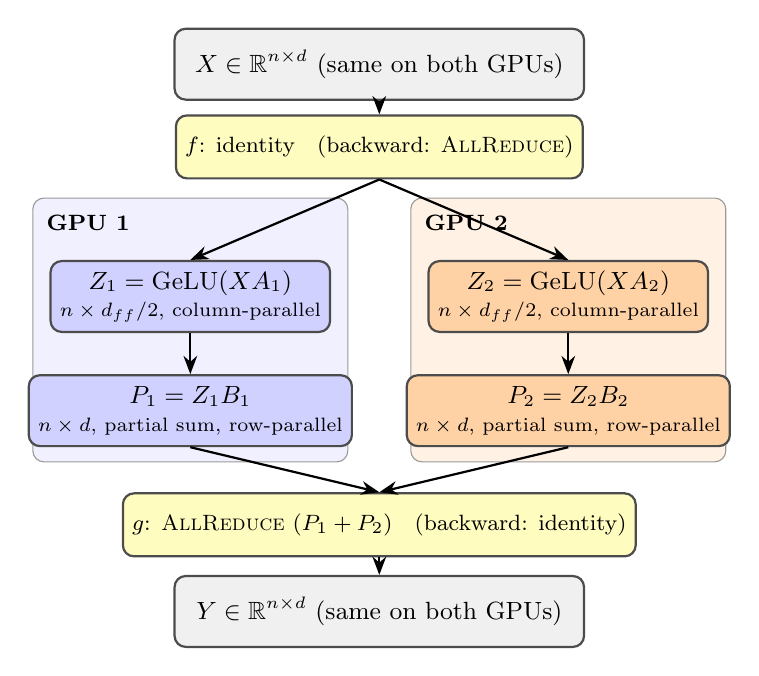
\begin{tikzpicture}[
    font=\small, >=Stealth,
    bx/.style={rectangle, rounded corners, draw=black!70, thick, align=center,
               minimum width=3.4cm, minimum height=0.9cm},
    op/.style={rectangle, rounded corners, draw=black!70, thick, fill=yellow!25,
               align=center, minimum width=4.4cm, minimum height=0.8cm,
               font=\footnotesize},
    arr/.style={-Stealth, thick}
]
  % GPU backgrounds
  \begin{scope}[on background layer]
    \fill[blue!6, draw=black!40, rounded corners] (-4.4,-5.05) rectangle (-0.4,-1.7);
    \fill[orange!10, draw=black!40, rounded corners] (0.4,-5.05) rectangle (4.4,-1.7);
  \end{scope}
  \node[font=\footnotesize\bfseries, anchor=north west] at (-4.35,-1.8) {GPU 1};
  \node[font=\footnotesize\bfseries, anchor=north west] at (0.45,-1.8) {GPU 2};

  \node[bx, fill=gray!12, minimum width=5.2cm] (X) at (0,0) {$X\in\mathbb{R}^{n\times d}$ (same on both GPUs)};
  \node[op] (f) at (0,-1.05) {$f$: identity \; (backward: \textsc{AllReduce})};

  \node[bx, fill=blue!18]   (a1) at (-2.4,-2.95) {$Z_1=\GeLU(XA_1)$\\[-1pt]{\scriptsize $n\times d_{ff}/2$, column-parallel}};
  \node[bx, fill=orange!35] (a2) at ( 2.4,-2.95) {$Z_2=\GeLU(XA_2)$\\[-1pt]{\scriptsize $n\times d_{ff}/2$, column-parallel}};
  \node[bx, fill=blue!18]   (b1) at (-2.4,-4.4) {$P_1=Z_1B_1$\\[-1pt]{\scriptsize $n\times d$, partial sum, row-parallel}};
  \node[bx, fill=orange!35] (b2) at ( 2.4,-4.4) {$P_2=Z_2B_2$\\[-1pt]{\scriptsize $n\times d$, partial sum, row-parallel}};

  \node[op] (g) at (0,-5.85) {$g$: \textsc{AllReduce} ($P_1+P_2$) \; (backward: identity)};
  \node[bx, fill=gray!12, minimum width=5.2cm] (Y) at (0,-6.95) {$Y\in\mathbb{R}^{n\times d}$ (same on both GPUs)};

  \draw[arr] (X) -- (f);
  \draw[arr] (f.south) -- (a1.north);
  \draw[arr] (f.south) -- (a2.north);
  \draw[arr] (a1) -- (b1);
  \draw[arr] (a2) -- (b2);
  \draw[arr] (b1.south) -- (g.north);
  \draw[arr] (b2.south) -- (g.north);
  \draw[arr] (g) -- (Y);
\end{tikzpicture}
\par\smallskip
{\small A tensor-parallel Transformer MLP on two GPUs: column-parallel
first layer, row-parallel second layer, one \textsc{AllReduce}.}
\end{center}

The same two operators are all one needs to implement the block. This
fragment (a sketch, in the spirit of the custom autograd functions of
Section~\ref{sec:autograd}) is a complete tensor-parallel MLP; each rank
stores only its own shard of $W_1$ and $W_2$:

\begin{lstlisting}
import torch, torch.nn as nn, torch.distributed as dist

class CopyToTP(torch.autograd.Function):      # "f"
    @staticmethod
    def forward(ctx, x):                      # identity
        return x
    @staticmethod
    def backward(ctx, grad):                  # all-reduce the gradient
        grad = grad.clone()
        dist.all_reduce(grad, op=dist.ReduceOp.SUM)
        return grad

class ReduceFromTP(torch.autograd.Function):  # "g"
    @staticmethod
    def forward(ctx, x):                      # all-reduce the output
        x = x.clone()
        dist.all_reduce(x, op=dist.ReduceOp.SUM)
        return x
    @staticmethod
    def backward(ctx, grad):                  # identity
        return grad

class TPMLP(nn.Module):
    def __init__(self, d, d_ff, tp):          # tp = #GPUs
        super().__init__()
        self.A = nn.Linear(d, d_ff // tp, bias=False)   # col shard of W1
        self.B = nn.Linear(d_ff // tp, d, bias=False)   # row shard of W2
    def forward(self, x):                     # x: [n, d], replicated
        x = CopyToTP.apply(x)
        z = torch.nn.functional.gelu(self.A(x))         # [n, d_ff/tp]
        p = self.B(z)                                   # partial sum
        return ReduceFromTP.apply(p)                    # summed
\end{lstlisting}

A useful unit test is to concatenate the shards of all ranks back into
dense $W_1$ and $W_2$ and check that the sharded output matches the dense
MLP.

\subsection{Attention: Split over Heads}

Multi-head attention is already ``cut into pieces'' by construction: head
$j$ computes its own $Q_j,K_j,V_j$ from its own slices of the projection
matrices, attends, and produces its own slice of the concatenated output.
Tensor parallelism simply hands different heads to different GPUs. The
$Q$, $K$, $V$ projections are column-parallel (each GPU owns the columns
belonging to its heads), the attention itself is purely local, and the
output projection $W_O$ is row-parallel (each GPU owns the rows that
consume its heads' outputs), so a single \textsc{AllReduce} suffices.

\begin{center}
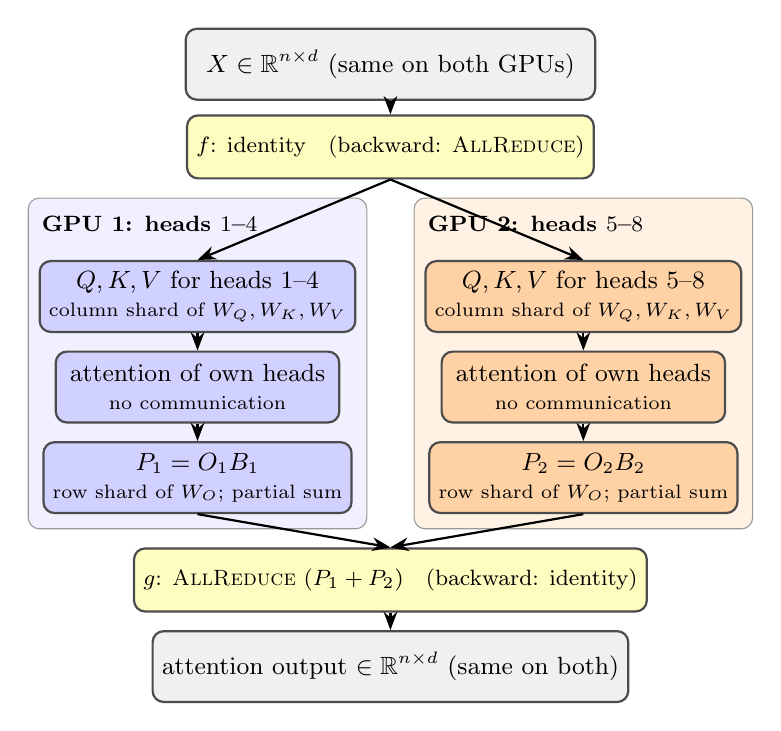
\begin{tikzpicture}[
    font=\small, >=Stealth,
    bx/.style={rectangle, rounded corners, draw=black!70, thick, align=center,
               minimum width=3.6cm, minimum height=0.9cm},
    op/.style={rectangle, rounded corners, draw=black!70, thick, fill=yellow!25,
               align=center, minimum width=4.4cm, minimum height=0.8cm,
               font=\footnotesize},
    arr/.style={-Stealth, thick}
]
  \begin{scope}[on background layer]
    \fill[blue!6, draw=black!40, rounded corners] (-4.6,-5.9) rectangle (-0.3,-1.7);
    \fill[orange!10, draw=black!40, rounded corners] (0.3,-5.9) rectangle (4.6,-1.7);
  \end{scope}
  \node[font=\footnotesize\bfseries, anchor=north west] at (-4.55,-1.8) {GPU 1: heads $1$--$4$};
  \node[font=\footnotesize\bfseries, anchor=north west] at (0.35,-1.8) {GPU 2: heads $5$--$8$};

  \node[bx, fill=gray!12, minimum width=5.2cm] (X) at (0,0) {$X\in\mathbb{R}^{n\times d}$ (same on both GPUs)};
  \node[op] (f) at (0,-1.05) {$f$: identity \; (backward: \textsc{AllReduce})};

  \node[bx, fill=blue!18]   (q1) at (-2.45,-2.95) {$Q,K,V$ for heads $1$--$4$\\[-1pt]{\scriptsize column shard of $W_Q,W_K,W_V$}};
  \node[bx, fill=orange!35] (q2) at ( 2.45,-2.95) {$Q,K,V$ for heads $5$--$8$\\[-1pt]{\scriptsize column shard of $W_Q,W_K,W_V$}};
  \node[bx, fill=blue!18]   (t1) at (-2.45,-4.1) {attention of own heads\\[-1pt]{\scriptsize no communication}};
  \node[bx, fill=orange!35] (t2) at ( 2.45,-4.1) {attention of own heads\\[-1pt]{\scriptsize no communication}};
  \node[bx, fill=blue!18]   (o1) at (-2.45,-5.25) {$P_1=O_1B_1$\\[-1pt]{\scriptsize row shard of $W_O$; partial sum}};
  \node[bx, fill=orange!35] (o2) at ( 2.45,-5.25) {$P_2=O_2B_2$\\[-1pt]{\scriptsize row shard of $W_O$; partial sum}};

  \node[op] (g) at (0,-6.55) {$g$: \textsc{AllReduce} ($P_1+P_2$) \; (backward: identity)};
  \node[bx, fill=gray!12, minimum width=5.2cm] (Y) at (0,-7.65) {attention output $\in\mathbb{R}^{n\times d}$ (same on both)};

  \draw[arr] (X) -- (f);
  \draw[arr] (f.south) -- (q1.north);
  \draw[arr] (f.south) -- (q2.north);
  \draw[arr] (q1) -- (t1); \draw[arr] (q2) -- (t2);
  \draw[arr] (t1) -- (o1); \draw[arr] (t2) -- (o2);
  \draw[arr] (o1.south) -- (g.north);
  \draw[arr] (o2.south) -- (g.north);
  \draw[arr] (g) -- (Y);
\end{tikzpicture}
\par\smallskip
{\small Tensor-parallel multi-head attention with $8$ heads on two GPUs;
the structure is identical to the MLP block, with ``heads'' playing the
role of ``hidden neurons''.}
\end{center}

Two practical constraints follow. The number of heads must be divisible
by the number of GPUs. With multi-query or grouped-query attention, where
there are fewer key/value heads than query heads, the tensor-parallel
degree cannot exceed the number of key/value heads without replicating
some of them.

\begin{example}[Per-layer cost of tensor parallelism with $t=4$ GPUs]
\label{ex:tp-cost}
Take a Transformer layer with model width $d=4096$, MLP width
$d_{ff}=4d=16384$, and $32$ attention heads of dimension $128$. Process a
micro-batch of $8$ sequences of $2048$ tokens, so $n=16384$ tokens, in
BF16 ($2$ bytes per number).

\emph{Parameters.} The MLP has $2\,d\,d_{ff}=134{,}217{,}728$ weights
($\approx134$\,M) and the attention block $4d^2=67{,}108{,}864$
($\approx67$\,M). With $t=4$, each GPU stores a quarter of each:
$\approx 33.6$\,M MLP weights and $\approx 16.8$\,M attention weights.
Concretely, in attention each GPU owns $8$ heads, i.e.\ column shards of
size $4096\times1024$ for each of $W_Q,W_K,W_V$ ($8\times128=1024$), and a
row shard of $W_O$ of size $1024\times4096$. In the MLP, $A_i$ is
$4096\times4096$ and $B_i$ is $4096\times4096$. Compute is divided by the
same factor $4$.

\emph{Communication.} Every \textsc{AllReduce} operates on a tensor of
shape $n\times d$, i.e.\ $16384\times4096\times2\ \text{B}\approx134$\,MB.
A ring \textsc{AllReduce} makes each GPU send $2\frac{t-1}{t}$ times the
tensor size, here $1.5\times134\approx201$\,MB. A layer needs two
\textsc{AllReduce} calls in the forward pass (after attention and after
the MLP) and two in the backward pass, so about $4\times201\approx0.8$\,GB
per GPU per layer, and roughly $26$\,GB per step for $32$ layers. The
volume scales with the number of tokens $n$ and with $d$, but \emph{not}
with the number of GPUs $t$ (beyond the factor $\tfrac{t-1}{t}$): adding
GPUs shrinks each GPU's compute and memory, while the communication per
GPU stays about the same.
\end{example}

This is the quantitative reason for the hardware rule in
Section~\ref{sec:tp-bandwidth}: on links with a few hundred GB/s per GPU
(NVLink inside a server), moving a few tens of gigabytes per step is
tolerable, whereas on links an order of magnitude slower (between
servers) the same traffic would dominate the step time.

\subsection{A Variant: Token-Sharded Activations}

In the formulation above, the activations $X$ and $Y$ are replicated on
all GPUs between blocks, so the operations between the blocks (residual
addition, dropout, $\LayerNorm$) are computed redundantly on every GPU.
The \textsc{AllReduce} can be traded for the two primitives it is made of
(Section~\ref{sec:collectives}): since $\AllReduce=\AllGather\circ
\ReduceScatter$, one may keep the activations \emph{sharded along the
token dimension} between blocks. Each GPU then holds only $n/t$ tokens of
every activation and performs the in-between operations on those tokens
alone. The block is bracketed by an \textsc{AllGather} before the
column-parallel layer (every GPU needs the full input) and by a
\textsc{ReduceScatter} after the row-parallel layer (sum the partial
results and hand each GPU its share of tokens). The total communication volume is the same as before.

\begin{center}
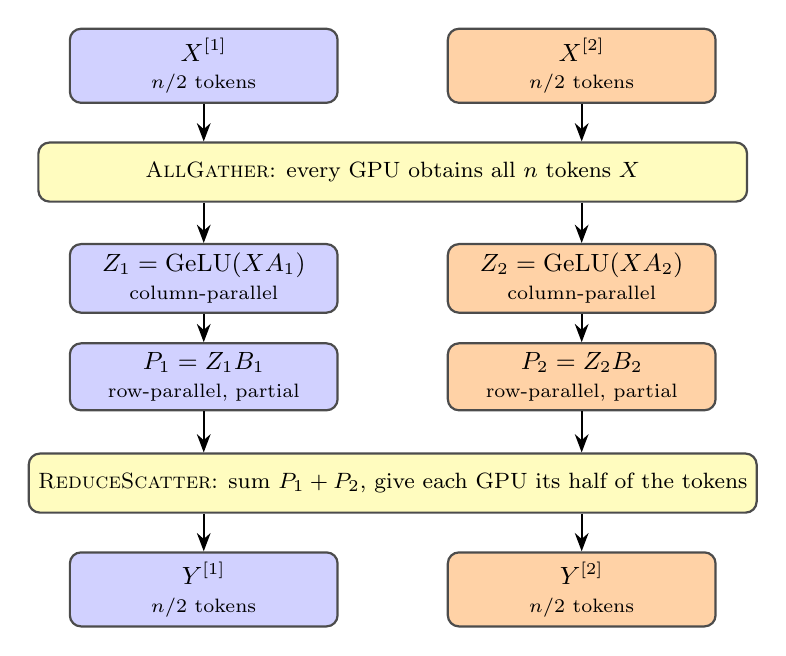
\begin{tikzpicture}[
    font=\small, >=Stealth,
    bx/.style={rectangle, rounded corners, draw=black!70, thick, align=center,
               minimum width=3.4cm, minimum height=0.85cm},
    wide/.style={rectangle, rounded corners, draw=black!70, thick, fill=yellow!25,
                 align=center, minimum width=9.0cm, minimum height=0.75cm,
                 font=\footnotesize},
    arr/.style={-Stealth, thick}
]
  \node[bx, fill=blue!18]   (x1) at (-2.4,0)  {$X^{[1]}$\\[-1pt]{\scriptsize $n/2$ tokens}};
  \node[bx, fill=orange!35] (x2) at ( 2.4,0)  {$X^{[2]}$\\[-1pt]{\scriptsize $n/2$ tokens}};
  \node[wide] (ag) at (0,-1.35) {\textsc{AllGather}: every GPU obtains all $n$ tokens $X$};
  \node[bx, fill=blue!18]   (a1) at (-2.4,-2.7) {$Z_1=\GeLU(XA_1)$\\[-1pt]{\scriptsize column-parallel}};
  \node[bx, fill=orange!35] (a2) at ( 2.4,-2.7) {$Z_2=\GeLU(XA_2)$\\[-1pt]{\scriptsize column-parallel}};
  \node[bx, fill=blue!18]   (b1) at (-2.4,-3.95) {$P_1=Z_1B_1$\\[-1pt]{\scriptsize row-parallel, partial}};
  \node[bx, fill=orange!35] (b2) at ( 2.4,-3.95) {$P_2=Z_2B_2$\\[-1pt]{\scriptsize row-parallel, partial}};
  \node[wide] (rs) at (0,-5.3) {\textsc{ReduceScatter}: sum $P_1+P_2$, give each GPU its half of the tokens};
  \node[bx, fill=blue!18]   (y1) at (-2.4,-6.65) {$Y^{[1]}$\\[-1pt]{\scriptsize $n/2$ tokens}};
  \node[bx, fill=orange!35] (y2) at ( 2.4,-6.65) {$Y^{[2]}$\\[-1pt]{\scriptsize $n/2$ tokens}};
  \draw[arr] (x1) -- (x1 |- ag.north); \draw[arr] (x2) -- (x2 |- ag.north);
  \draw[arr] (a1 |- ag.south) -- (a1); \draw[arr] (a2 |- ag.south) -- (a2);
  \draw[arr] (a1) -- (b1); \draw[arr] (a2) -- (b2);
  \draw[arr] (b1) -- (b1 |- rs.north); \draw[arr] (b2) -- (b2 |- rs.north);
  \draw[arr] (y1 |- rs.south) -- (y1); \draw[arr] (y2 |- rs.south) -- (y2);
\end{tikzpicture}
\par\smallskip
{\small The same MLP block with token-sharded activations: the
\textsc{AllReduce} of the previous figure is replaced by a
\textsc{ReduceScatter} at the end and a matching \textsc{AllGather} at the
start of the next block. (This sharding of the token dimension is distinct
from the long-context sequence-parallel methods of the next section.)}
\end{center}

\subsection{Distributed LayerNorm}

If the \emph{feature} dimension of an activation is itself sharded, then
$\LayerNorm$ needs global statistics (mean and variance) computed across
GPUs. Each device computes local partial sums $\sum_i x_i$ and
$\sum_i x_i^2$; a single \textsc{AllReduce} of these two numbers per token
yields the global moments from which the normalised activations follow.

\begin{example}[Distributed statistics for one token]
Let a token have four features $x=(1,2,3,4)$, with GPU~1 holding $(1,2)$
and GPU~2 holding $(3,4)$. Locally,
GPU~1 computes $\sum x=3$, $\sum x^2=5$ and GPU~2 computes $\sum x=7$,
$\sum x^2=25$. After an \textsc{AllReduce} both hold $\sum x=10$ and
$\sum x^2=30$, hence
\[
\mu=\frac{10}{4}=2.5,\qquad
\sigma^2=\frac{30}{4}-\mu^2=7.5-6.25=1.25,
\]
which are exactly the mean and variance of $(1,2,3,4)$. Each GPU then
normalises its own two features with these values. Only two scalars per
token cross the network, so this is cheap compared to the
$n\times d$ tensors of the matrix products.
\end{example}

In the Megatron-style formulation above the residual stream is replicated,
so each GPU already holds all $d$ features of its tokens and
$\LayerNorm$ needs no communication at all; the sharded-statistics case
arises when features (rather than tokens) are distributed.

\label{sec:tp-bandwidth}

\begin{remark}
Tensor parallelism is \emph{communication-intensive}. Every forward pass
through every layer entails at least one collective operation (two per
layer, as counted above), and they sit on the critical path: the next
matrix product cannot start before the \textsc{AllReduce} finishes. For
this reason tensor parallelism is typically confined to the GPUs within a
single server, interconnected by high-bandwidth NVLink; pipeline or data
parallelism handles inter-server scaling.
\end{remark}

For a minimalistic way to try tensor parallelism in PyTorch, one can use the
\href{...}{\texttt{tensor\_parallel}}
package (\texttt{pip install tensor\_parallel}).

%%%%%%%%%%%%%%%%%%%%%%%%%%%%%%%%%%%%%%%%%%%%%%%%%%%%%%%%%%%%%%%%%%%%%%%%
\section{Sequence Parallelism}
%%%%%%%%%%%%%%%%%%%%%%%%%%%%%%%%%%%%%%%%%%%%%%%%%%%%%%%%%%%%%%%%%%%%%%%%

\subsection{Motivation: The Tyranny of $L^2$}

The self-attention score matrix is of shape $L \times L$ in the sequence
length, so both memory and compute grow as $O(L^2 d)$. For million-token
contexts, even storing the activations of a \emph{single} sequence on a
single device becomes impossible. Tensor parallelism addresses ``too many
weights''; sequence parallelism addresses ``too long a sequence.'' The
goal is to avoid storing all activations on every device.

\subsection{DeepSpeed-Ulysses}

The DeepSpeed-Ulysses design
(\href{https://arxiv.org/abs/2309.14509}{arXiv:2309.14509}) partitions the
sequence dimension $L$ across $P$ devices, so each holds a slice of length
$L/P$. The MLP layers require no modification---they are token-parallel.
The attention layer, however, requires global information across the
sequence. The trick is to convert between partitions:

\begin{enumerate}[leftmargin=1.8em, itemsep=2pt]
    \item Each device locally computes $Q, K, V$ projections on its
    sequence shard.
    \item An \textsc{AllToAll} redistributes so that each device holds
    \emph{all} of the sequence but only a subset of the \emph{attention
    heads}.
    \item The standard attention computation proceeds head-wise.
    \item A second \textsc{AllToAll} restores the sequence-parallel layout
    for the subsequent MLP.
\end{enumerate}

\begin{center}
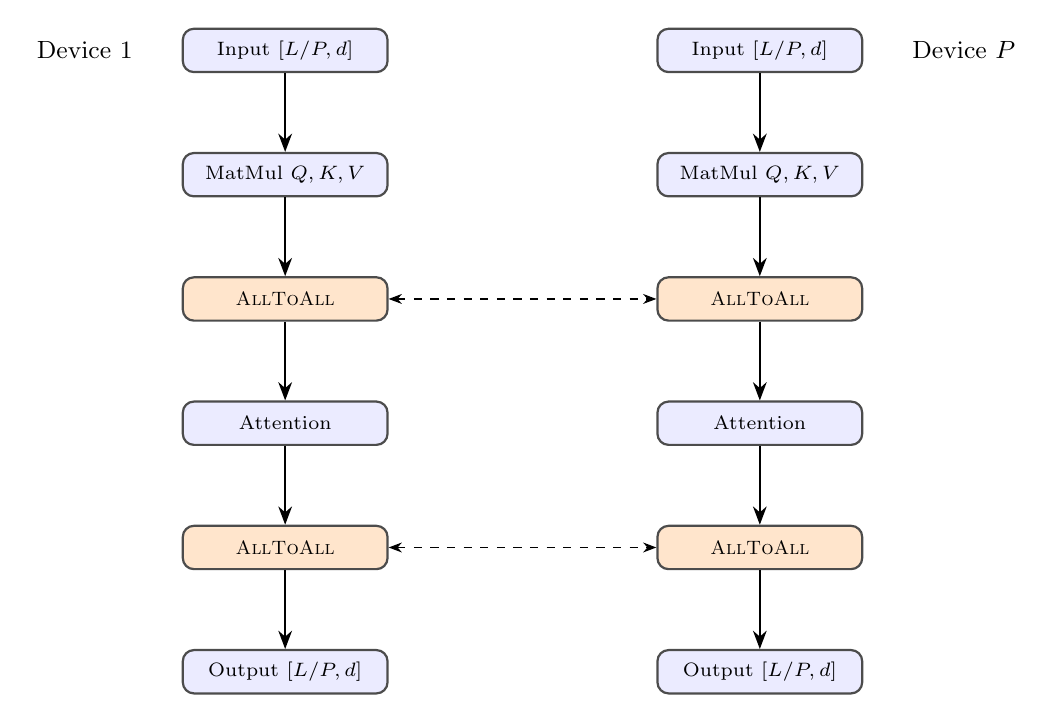
\begin{tikzpicture}[
    node distance=1.0cm, font=\scriptsize, >=Stealth,
    box/.style={rectangle, rounded corners, draw=black!70, thick, fill=blue!8,
                minimum width=2.6cm, minimum height=0.55cm, align=center},
    comm/.style={rectangle, rounded corners, draw=black!70, thick, fill=orange!20,
                 minimum width=2.6cm, minimum height=0.55cm, align=center},
    arr/.style={-Stealth, thick}
]
    % Device 1
    \node (in1) [box] {Input $[L/P, d]$};
    \node (qkv1) [box, below=of in1] {MatMul $Q,K,V$};
    \node (all1) [comm, below=of qkv1] {\textsc{AllToAll}};
    \node (at1) [box, below=of all1] {Attention};
    \node (all2) [comm, below=of at1] {\textsc{AllToAll}};
    \node (out1) [box, below=of all2] {Output $[L/P, d]$};
    \draw[arr] (in1)--(qkv1); \draw[arr] (qkv1)--(all1);
    \draw[arr] (all1)--(at1); \draw[arr] (at1)--(all2); \draw[arr] (all2)--(out1);
    % Device P
    \node (inP) [box, right=3.4cm of in1] {Input $[L/P, d]$};
    \node (qkvP) [box, below=of inP] {MatMul $Q,K,V$};
    \node (allP1) [comm, below=of qkvP] {\textsc{AllToAll}};
    \node (atP) [box, below=of allP1] {Attention};
    \node (allP2) [comm, below=of atP] {\textsc{AllToAll}};
    \node (outP) [box, below=of allP2] {Output $[L/P, d]$};
    \draw[arr] (inP)--(qkvP); \draw[arr] (qkvP)--(allP1);
    \draw[arr] (allP1)--(atP); \draw[arr] (atP)--(allP2); \draw[arr] (allP2)--(outP);
    \draw[dashed, <->] (all1) -- (allP1);
    \draw[dashed, <->] (all2) -- (allP2);
    \node[font=\small, left=0.5cm of in1] {Device 1};
    \node[font=\small, right=0.5cm of inP] {Device $P$};
\end{tikzpicture}
\end{center}

\subsection{Ring Attention and Its Relatives}

Besides Ulysses, several other methods belong under this heading:
\begin{itemize}[leftmargin=1.5em, itemsep=2pt]
    \item an early mention of parallelism over sequences
          (\href{https://arxiv.org/abs/2105.05720}{arXiv:2105.05720});
    \item \textsc{Ring Attention}
          (\href{https://arxiv.org/abs/2310.01889}{arXiv:2310.01889}),
          which computes attention dot products and softmax in parallel;
    \item \textsc{Flux}
          (\href{https://arxiv.org/abs/2406.06858}{arXiv:2406.06858}),
          which overlaps computation and communication with custom
          kernels.
\end{itemize}

In \textsc{Ring Attention} the sequence is chunked into blocks that are
passed around a ring of devices, each computing a block of the $QK^\top$
product and accumulating a running softmax. The communication pattern is
point-to-point rather than global, and overlaps neatly with computation.
\textsc{Flux} employs custom kernels that overlap computation with
communication at the tile level, minimising idle time on the accelerator.

\begin{remark}
Neither sequence parallelism nor \textsc{FlashAttention} changes the
\emph{mathematics} of the model. Both alter the \emph{schedule and
locality} of the computation. The forward pass is bit-identical (up to
floating-point non-associativity) to a monolithic implementation.
\end{remark}

%%%%%%%%%%%%%%%%%%%%%%%%%%%%%%%%%%%%%%%%%%%%%%%%%%%%%%%%%%%%%%%%%%%%%%%%
\section{Mixture of Experts and Expert Parallelism}
%%%%%%%%%%%%%%%%%%%%%%%%%%%%%%%%%%%%%%%%%%%%%%%%%%%%%%%%%%%%%%%%%%%%%%%%

\subsection{Sparse Conditional Computation}

The \emph{Mixture of Experts} (MoE) architecture replaces a dense
feed-forward layer with a collection of \emph{experts}
$\{E_1, \ldots, E_n\}$ and a small \emph{gating network} $G(x)$ that
routes each input $x$ to a subset of them:
\begin{equation}
y = \sum_{i=1}^{n} g_i(x) \cdot E_i(x),
\qquad
g(x) = \mathrm{top}\text{-}k\!\left(\softmax(G(x))\right).
\end{equation}
Because only $k \ll n$ experts are active per token, the FLOPs per token
remain constant while the \emph{capacity} of the model (its total
parameter count) scales linearly with the number of experts.

\begin{center}
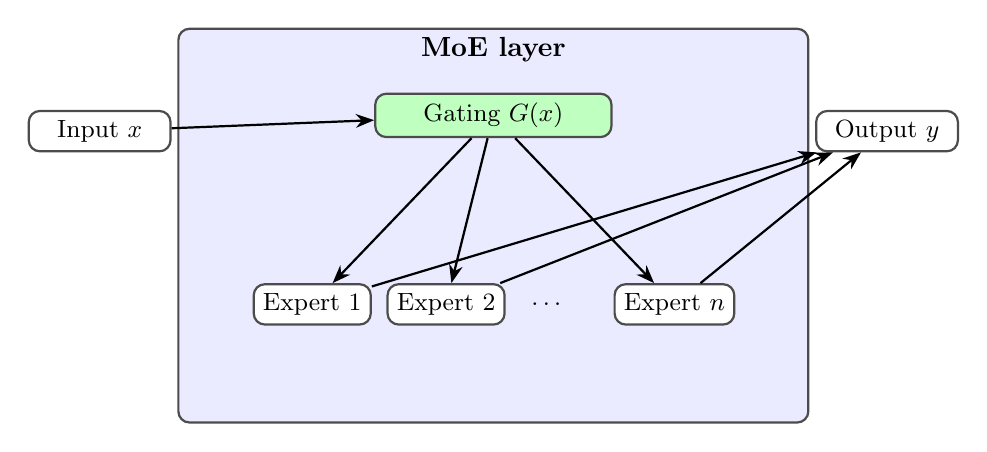
\begin{tikzpicture}[node distance=0.9cm, >=Stealth, font=\small,
    bx/.style={rectangle, rounded corners, draw=black!70, thick, fill=white}]
    \node[rectangle, rounded corners, draw=black!70, thick, fill=blue!8,
          minimum width=8cm, minimum height=5cm] (moe) at (0,0) {};
    \node[anchor=north, font=\bfseries] at (moe.north) {MoE layer};
    \node[bx, minimum width=1.8cm] (input) at (-5, 1.2) {Input $x$};
    \node[bx, minimum width=1.8cm] (output) at (5, 1.2) {Output $y$};
    \node[bx, fill=green!25, minimum width=3cm] (gate) at (0, 1.4) {Gating $G(x)$};
    \node[bx] (e1) at (-2.3, -1) {Expert 1};
    \node[bx] (e2) at (-0.6, -1) {Expert 2};
    \node at (0.7, -1) {$\dots$};
    \node[bx] (en) at (2.3, -1) {Expert $n$};
    \draw[-Stealth, thick] (input) -- (gate);
    \draw[-Stealth, thick] (gate) -- (e1); \draw[-Stealth, thick] (gate) -- (e2); \draw[-Stealth, thick] (gate) -- (en);
    \draw[-Stealth, thick] (e1) -- (output); \draw[-Stealth, thick] (e2) -- (output); \draw[-Stealth, thick] (en) -- (output);
\end{tikzpicture}
\end{center}

The idea originates with Shazeer et al.\
(\href{https://arxiv.org/pdf/1701.06538.pdf}{arXiv:1701.06538}) and
underlies contemporary MoE models such as Mixtral and DeepSeek-V3. For
MoE training in practice, see
\href{https://github.com/databricks/megablocks}{Megablocks}.

\subsection{Expert Parallelism}

Naturally, if there are $n$ experts and $D$ devices, one distributes the
experts across devices: $n/D$ experts per GPU. This is \emph{expert
parallelism}. Routing a token to its chosen experts requires an
\textsc{AllToAll} exchange: each device sends the tokens assigned to
remote experts away, receives its own tokens back after expert
processing, and reassembles them.

\subsection{Load Balancing and the Switch Transformer}

MoE training faces a pathology: the gating network may collapse onto a
few experts, starving the rest of gradient signal. The Switch Transformer
(\href{https://arxiv.org/pdf/2101.03961.pdf}{arXiv:2101.03961}) is a
prominent MoE variant; countermeasures include:

\begin{itemize}[leftmargin=1.5em, itemsep=2pt]
    \item \textbf{Capacity limits.} Each expert processes at most
    \begin{equation}
    \text{Expert Capacity} = \left\lfloor \frac{\text{Tokens per batch}}{n_{\text{experts}}}
    \right\rfloor \cdot \text{Capacity Factor},
    \end{equation}
    above which tokens are dropped---the MoE analogue of dropout.
    \item \textbf{Load-balancing loss.} An auxiliary term penalises
    imbalance between the chosen experts.
    \item \textbf{Noise injection.} Additive noise on gating logits
    encourages exploration during training.
\end{itemize}

\subsection{Overlap of Computation and Communication}

The Switch Transformer reduces the bubble introduced by the
\textsc{AllToAll} by dividing forward and backward MLP computation into
smaller chunks and interleaving them with dispatch / combine
communication. Computation on one chunk overlaps communication of the
next, so the accelerator stays saturated.

%%%%%%%%%%%%%%%%%%%%%%%%%%%%%%%%%%%%%%%%%%%%%%%%%%%%%%%%%%%%%%%%%%%%%%%%
\section{Fully Sharded Data Parallelism (FSDP) / ZeRO}
%%%%%%%%%%%%%%%%%%%%%%%%%%%%%%%%%%%%%%%%%%%%%%%%%%%%%%%%%%%%%%%%%%%%%%%%

Naive data parallelism replicates every parameter, every gradient, and
every optimizer state on every device---a profligate use of memory.
\textsc{ZeRO} (Rajbhandari et al.; see Microsoft's
\href{https://www.microsoft.com/en-us/research/blog/zero-deepspeed-new-system-optimizations-enable-training-models-with-over-100-billion-parameters/}{announcement
post}) and the PyTorch equivalent \emph{Fully Sharded Data Parallelism}
(FSDP;
\href{https://pytorch.org/blog/introducing-pytorch-fully-sharded-data-parallel-api/}{PyTorch
blog post}) shard these quantities \emph{across} the data-parallel
workers, reconstructing them on the fly.

\subsection{Four-way ZeRO training}

Consider four GPUs, each holding a shard of the model
$\{M_0, M_1, M_2, M_3\}$ and a shard of the batch
$\{D_0, D_1, D_2, D_3\}$. At any moment each GPU owns:

\begin{itemize}[leftmargin=1.5em, itemsep=2pt]
    \item Its \textbf{FP32 master weights} $\theta^{(i)}$ (one quarter of
    the total).
    \item Its \textbf{FP32 optimizer statistics} $m^{(i)}, v^{(i)}$ (one
    quarter).
    \item Its \textbf{FP16 gradient shard} $\grad \theta^{(i)}$ (one
    quarter).
\end{itemize}

To execute the forward pass through layer $\ell$, \emph{the GPU owning
that layer's shard broadcasts it to the others} via an
\textsc{AllGather}. All GPUs then perform the forward on their respective
data; the broadcast shard is discarded from non-owners immediately after
use. The backward pass is symmetric: an \textsc{AllGather} to fetch the
shard, compute local gradient contributions, then a
\textsc{ReduceScatter} to return each GPU's share of the gradient.

\begin{center}
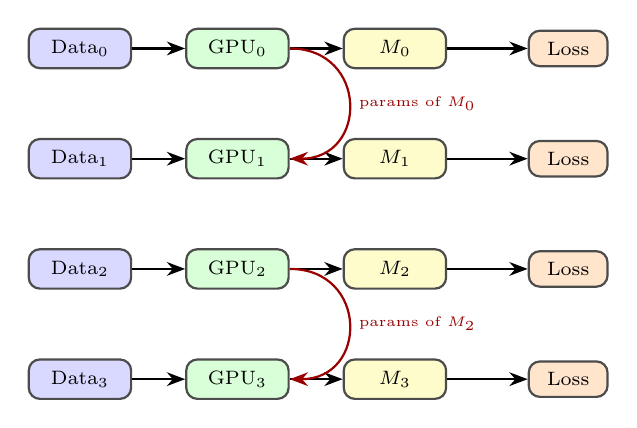
\begin{tikzpicture}[
    >=Stealth, font=\scriptsize,
    data/.style={rectangle, rounded corners, draw=black!70, thick, fill=blue!15, minimum width=1.3cm, minimum height=0.5cm},
    mod/.style={rectangle, rounded corners, draw=black!70, thick, fill=yellow!20, minimum width=1.3cm, minimum height=0.5cm},
    gpu/.style={rectangle, rounded corners, draw=black!70, thick, fill=green!15, minimum width=1.3cm, minimum height=0.5cm},
    loss/.style={rectangle, rounded corners, draw=black!70, thick, fill=orange!20, minimum width=1cm, minimum height=0.45cm}
]
    \foreach \i/\y in {0/1.4, 1/0, 2/-1.4, 3/-2.8} {
        \node[data] (d\i) at (-5, \y) {Data$_\i$};
        \node[gpu]  (g\i) at (-3, \y) {GPU$_\i$};
        \node[mod]  (m\i) at (-1, \y) {$M_\i$};
        \node[loss] (L\i) at (1.2, \y) {Loss};
        \draw[-Stealth, thick] (d\i)--(g\i);
        \draw[-Stealth, thick] (g\i)--(m\i);
        \draw[-Stealth, thick] (m\i)--(L\i);
    }
    \draw[-Stealth, thick, red!60!black] (g0.east) .. controls +(right:1cm) and +(right:1cm) ..
        node[midway, right, font=\tiny] {params of $M_0$} (g1.east);
    \draw[-Stealth, thick, red!60!black] (g2.east) .. controls +(right:1cm) and +(right:1cm) ..
        node[midway, right, font=\tiny] {params of $M_2$} (g3.east);
\end{tikzpicture}
\end{center}

\begin{observation}
The pattern of \emph{computation} resembles data parallelism (each GPU
processes its own data), but the \emph{storage} of weights resembles
pipeline parallelism (only one GPU owns each shard at rest). The
essential novelty is that weights are transiently broadcast on demand
rather than statically replicated.
\end{observation}

\subsection{Relationship to Offloading}

FSDP and parameter offloading are distinct:
\begin{itemize}[leftmargin=1.5em, itemsep=2pt]
    \item \textbf{Offloading} moves parameters between GPU and CPU over
    PCIe.
    \item \textbf{FSDP} moves parameters between GPUs over NVLink /
    InfiniBand, which is one to two orders of magnitude faster.
\end{itemize}
FSDP is therefore the first-line strategy in multi-GPU settings;
offloading remains for single-GPU or extreme-scale scenarios.

\subsection{Implementations}

The practical options are:
\begin{itemize}[leftmargin=1.5em, itemsep=2pt]
    \item \href{https://www.deepspeed.ai/}{DeepSpeed}: sharded data
          parallelism, offloading (see the
          \href{https://www.deepspeed.ai/news/2021/03/07/zero3-offload.html}{ZeRO-3
          Offload post}), and tensor parallelism, under active
          development. The same techniques also power
          \emph{DeepSpeed Inference}
          (\href{https://arxiv.org/abs/2207.00032}{arXiv:2207.00032}):
          offloading, tensor and pipeline parallelism, ``and a ton of
          hacks.''
    \item \textbf{FSDP}: most of DeepSpeed's features behind a native
          PyTorch API.
    \item \textbf{Model-specific implementations}, such as
          \href{https://github.com/NVIDIA/Megatron-LM}{Megatron-LM}.
\end{itemize}

%%%%%%%%%%%%%%%%%%%%%%%%%%%%%%%%%%%%%%%%%%%%%%%%%%%%%%%%%%%%%%%%%%%%%%%%
\section{Automated Parallelism}
%%%%%%%%%%%%%%%%%%%%%%%%%%%%%%%%%%%%%%%%%%%%%%%%%%%%%%%%%%%%%%%%%%%%%%%%

The material in this section follows the ICML~2022 tutorial on big
models.\footnote{\url{https://sites.google.com/view/icml-2022-big-model}}

\subsection{From Asset-Centric to Operation-Centric Views}

\begin{definition}[Classic view]
\textbf{Data parallelism} partitions data; \textbf{model parallelism}
partitions parameters.
\end{definition}

\begin{definition}[Modern view]
\textbf{Inter-op parallelism} partitions distinct computational nodes
(e.g., an image encoder and a text encoder run concurrently).
\textbf{Intra-op parallelism} partitions a single operation (e.g., a
large matrix multiplication is split across devices along one of its
axes).
\end{definition}

\subsection{Learned and Optimization-Based Partitioning}

Before Alpa, two lines of work tackled the partitioning problem directly:
\emph{RL-based} partitioning, exemplified by
\href{https://people.csail.mit.edu/hongzi/content/publications/placeto-neurips19.pdf}{Placeto},
and \emph{optimization-based} partitioning
(\href{https://arxiv.org/abs/2006.16423}{arXiv:2006.16423}).

\subsection{Alpa and the Compiler View}

\textsc{Alpa} (\href{https://arxiv.org/abs/2201.12023}{arXiv:2201.12023})
combines optimization-based partitioning with a reduced search space. It
treats parallelisation as a \emph{graph partitioning and scheduling
problem}: given a computational graph and a device cluster, Alpa uses
dynamic programming for inter-op scheduling and integer linear
programming for intra-op sharding. The user writes a JAX function; Alpa
maps it to the cluster.

\begin{center}
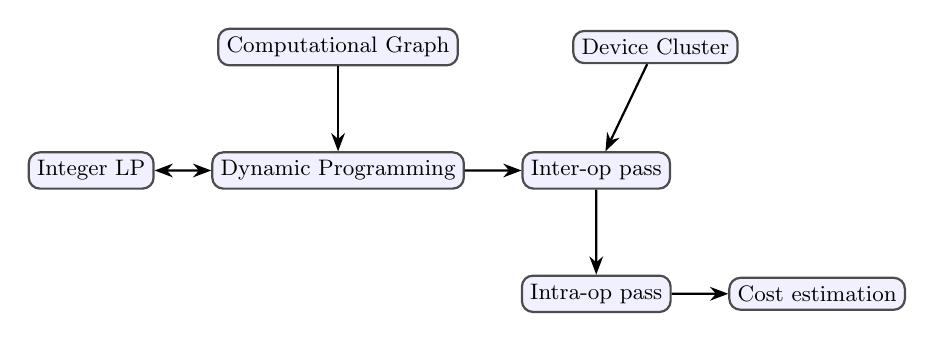
\begin{tikzpicture}[
    node distance=1.2cm, >=Stealth, font=\small, scale=0.9, transform shape,
    bx/.style={rectangle, rounded corners, draw=black!70, thick, fill=blue!6},
    arr/.style={-Stealth, thick}
]
    \node[bx, minimum width=3.2cm] (CG) {Computational Graph};
    \node[bx, right=1.6cm of CG] (DC) {Device Cluster};
    \node[bx, below=of CG] (DP) {Dynamic Programming};
    \node[bx, left=0.8cm of DP] (ILP) {Integer LP};
    \node[bx, right=0.8cm of DP] (IP) {Inter-op pass};
    \node[bx, below=of IP] (IOP) {Intra-op pass};
    \node[bx, right=0.8cm of IOP] (CE) {Cost estimation};
    \draw[arr] (CG)--(DP); \draw[arr] (DC)--(IP);
    \draw[arr] (DP)--(IP); \draw[arr] (IP)--(IOP); \draw[arr] (IOP)--(CE);
    \draw[Stealth-Stealth, thick] (ILP)--(DP);
\end{tikzpicture}
\end{center}

Alpa was not the first algorithm for automatic parallelism, but it was
the first that is usable (most of the time). It was deprecated in 2024,
but successors exist: in JAX, use \texttt{pjit}/\texttt{xmap} with
improved XLA optimisations; in PyTorch, see
\href{https://docs.pytorch.org/xla/master/spmd.html}{XLA SPMD}. For
standard models, DeepSpeed is often enough.

The broader trend is away from bespoke frameworks and towards
compiler-driven solutions---JAX with XLA, PyTorch with XLA SPMD and
\texttt{torch.compile}---in which parallelism is specified declaratively
through sharding annotations on a mesh.

\subsection{Combined Strategies}

\begin{remark}[Hierarchical parallelism]
In production, one first forms a \emph{model-parallel group}: the
smallest set of GPUs onto which the model fits via tensor and/or pipeline
parallelism. Multiple such groups are then orchestrated via data
parallelism. The hybrid of these three axes---plus checkpointing,
offloading, and (sometimes) expert parallelism---constitutes the state of
the art.
\end{remark}

%%%%%%%%%%%%%%%%%%%%%%%%%%%%%%%%%%%%%%%%%%%%%%%%%%%%%%%%%%%%%%%%%%%%%%%%
\section{Under the Hood: PyTorch Autograd and Custom Functions}
\label{sec:autograd}
%%%%%%%%%%%%%%%%%%%%%%%%%%%%%%%%%%%%%%%%%%%%%%%%%%%%%%%%%%%%%%%%%%%%%%%%

Every idea in the preceding sections is ultimately expressed as a
\texttt{torch.autograd.Function}. A brief excursion into its internals is
in order.

\subsection{The Role of \texttt{ctx}}

The context object passed to each \texttt{forward} / \texttt{backward}
method is a per-call scratchpad in which tensors required for the
backward pass are saved. Without it, the chain rule has nowhere to find
the local Jacobians.

\subsection{A Custom Function}

\begin{lstlisting}
import torch
import torch.nn as nn

class MyFunc(torch.autograd.Function):

    @staticmethod
    def forward(ctx, fn, calldata, x):
        ctx.save_for_backward(x)
        ctx.fn = fn
        return fn(x)

    @staticmethod
    def backward(ctx, grad_out):
        (x,) = ctx.saved_tensors
        fn = ctx.fn
        # local Jacobian happens to be 2 * fn(x) in this toy example
        return None, None, grad_out * 2 * fn(x)
\end{lstlisting}

The chain rule is applied explicitly:
\begin{equation}
\frac{\partial \LL}{\partial x} =
\frac{\partial \LL}{\partial z} \cdot \frac{\partial z}{\partial x}.
\end{equation}
Non-tensor arguments (\texttt{fn}, \texttt{calldata}) receive
\texttt{None} in the gradient tuple.

\subsection{Checkpointing as a Custom Function}

Gradient checkpointing is realised in PyTorch by wrapping a subgraph's
forward in \verb|torch.no_grad()|, saving only the RNG state and the
inputs, and re-invoking the subgraph's forward with
\verb|torch.enable_grad()| during the backward pass---exactly the
trade-off of Section~\ref{sec:ckpt}.

\subsection{A Distributed \texttt{AllReduce} Module}

\begin{lstlisting}
import torch
import torch.nn as nn
import torch.distributed as dist

class AllReduceModule(nn.Module):
    def forward(self, x):
        dist.all_reduce(x, op=dist.ReduceOp.SUM)
        return x
\end{lstlisting}

The module is deceptively simple, but it is the seam at which the
communication graph meets the computational graph. (The operators $f$ and
$g$ of tensor parallelism in Section~\ref{sec:tp} are exactly this seam,
with the backward pass written out explicitly.)

\subsection{Offloading as a Custom Function}

An offloading wrapper extends the pattern by moving the saved tensor from
GPU to CPU inside \texttt{forward}, and back to GPU at the start of
\texttt{backward}. One may similarly \emph{quantise} activations in
\texttt{forward} and dequantise in \texttt{backward}.

\begin{remark}
Hooks (\texttt{register\_forward\_hook},
\texttt{register\_backward\_hook}) are the tool of choice for diagnostic
instrumentation. They are \emph{not} a substitute for custom autograd
functions in production: because \texttt{torch.compile} may rewrite the
graph, hooks attached to the pre-compilation structure can silently be
bypassed.
\end{remark}

%%%%%%%%%%%%%%%%%%%%%%%%%%%%%%%%%%%%%%%%%%%%%%%%%%%%%%%%%%%%%%%%%%%%%%%%
\section{A Decision Procedure}
%%%%%%%%%%%%%%%%%%%%%%%%%%%%%%%%%%%%%%%%%%%%%%%%%%%%%%%%%%%%%%%%%%%%%%%%

Given a model and a cluster, the following schematic captures the
practical logic of choice.

\begin{enumerate}[leftmargin=1.8em, itemsep=2pt]
    \item \emph{Batch too large?} $\Rightarrow$ Gradient accumulation.
    \item \emph{Activations too large?} $\Rightarrow$ Gradient
    checkpointing.
    \item \emph{Parameters too large for one GPU, but cluster is small
    and well-connected?} $\Rightarrow$ Tensor parallelism within a
    server; data parallelism across servers.
    \item \emph{Parameters too large, cluster is poorly connected?}
    $\Rightarrow$ Pipeline parallelism (1F1B or zero-bubble), possibly
    combined with checkpointing.
    \item \emph{Parameters exceed the aggregate memory of the cluster?}
    $\Rightarrow$ FSDP / ZeRO, combined with CPU offloading of optimizer
    states.
    \item \emph{Context length is extreme?} $\Rightarrow$ Sequence
    parallelism (DeepSpeed-Ulysses, Ring Attention).
    \item \emph{Total capacity must scale without proportional FLOPs?}
    $\Rightarrow$ Mixture of Experts with expert parallelism.
    \item \emph{Single GPU available and model too large?} $\Rightarrow$
    Parameter offloading with L2L-style pre-fetching.
\end{enumerate}

No single axis suffices for frontier models; the competent engineer
learns to combine them.

\end{document}